\documentclass[twoside,11pt]{article}

% Any additional packages needed should be included after jmlr2e.
% Note that jmlr2e.sty includes epsfig, amssymb, natbib and graphicx,
% and defines many common macros, such as 'proof' and 'example'.
%
% It also sets the bibliographystyle to plainnat; for more information on
% natbib citation styles, see the natbib documentation, a copy of which
% is archived at http://www.jmlr.org/format/natbib.pdf

\usepackage{jmlr2e}
\usepackage{amsmath}
\usepackage{pgfplots}
% and optionally (as of Pgfplots 1.3):
\pgfplotsset{compat=newest}
\pgfplotsset{plot coordinates/math parser=false}
\newlength\figureheight
\newlength\figurewidth

% Definitions of handy macros can go here

\newcommand{\dataset}{{\cal D}}
\newcommand{\fracpartial}[2]{\frac{\partial #1}{\partial  #2}}

% Heading arguments are {volume}{year}{pages}{submitted}{published}{author-full-names}

\jmlrheading{1}{2015}{1-48}{4/15}{10/15}{Wouter Kouw}

% Short headings should be running head and authors last names

\ShortHeadings{Feature Importance Regularization}{Kouw, Krijthe, Loog \& Van der Maaten}
\firstpageno{1}

\def\ci{\perp\!\!\!\perp}

\begin{document}

\title{Feature Importance Regularization \\ for domain adaptation}

\author{\name Wouter Kouw \email W.M.Kouw@tudelft.nl \\
       Delft University of Technology
       \AND
       \name Jesse Krijthe \email J.H.Krijthe@tudelft.nl \\
       Delft University of Technology  \\
       Leiden University Medical Center
       \AND
       \name Marco Loog \email M.Loog@tudelft.nl \\
       Delft University of Technology \\
       University of Copenhagen
       \AND
       \name Laurens van der Maaten \email L.J.P.Vandermaaten@tudelft.nl \\
       Delft University of Technology \\
       Facebook Research
}

\editor{Leslie Pack Kaelbling}

\maketitle

\begin{abstract}%   <- trailing '%' for backward compatibility of .sty file
Domain adaptation is a supervised learning problem where the training and test data come from different distributions. In this paper we study a classifier that assumes a particular dependence between two domains. Modeling that dependence with a conditional Bernoulli	 distribution leads to adapting to the relative frequency of feature presence. We show that if the model is correct, the adapted classifier is equivalent to the target classifier. Applying it to real-world datasets shows that it competes well with popular linear adapted classifiers.
\end{abstract}

\begin{keywords}
Domain adaptation, transfer learning, covariate shift, empirical risk minimization, data-dependent regularization, dropout.
\end{keywords}

\section{Introduction}

In supervised learning, classifiers learn from labeled samples and predict labels of new samples. It is implicitly assumed that these new samples come from the same distribution as the already observed ones. However, this assumption often does not hold. For example, a classifier that has learned to recognize speech from sound fragments of one person can not easily recognize a different person's sound fragments, because the fragments of two different people have different statistics [\cite{leggetter1995maximum}]. 

A common occurence of this problem is when we have a specific method of gathering data to study a problem. Classifiers trained on these measurements do not generalize to other acquisition methods. For example, training an image segmentation classifier on data from one MRI scanner does not imply that it will perform well on data from a different scanner  [\cite{van2013transfer}]. The scanning protocols and mechanical specifications ensure that the intensity values are distributed differently over voxels.
Another example is object recognition in computer vision [\cite{saenko2010adapting}]. If the images available to us for training have been taken with one camera and for testing with another camera, then the pixel intensity distributions may differ due to lens or exposure settings.
In natural language processing it is hard to classify movie reviews after training on tweets due to different probabilities of using informal words [\cite{peddinti2011domain}]. As for bioinformatics, integrating genome sequence data from multiple acquisition centers can also be considered a domain adaptation problem, because cells are subject to different laboratory conditions [\cite{borgwardt2006integrating}]. 

In each of these cases there is a bias in the data sampling procedure, leading to different probabilities over the same events which we refer to as domains. Domain adaptation is the task of adapting a classifier trained on one or more source domains such that it generalizes to a target domain. 

We consider having target labels available during training a multi-task learning problem [\cite{pan2010survey, moreno2012unifying}] and requesting a small number of target labels an active learning problem [\cite{cohn1996active}]. If the distribution of the target samples changes for small batches, then we consider this an online learning problem [\cite{ma2009identifying}]. 

Sometimes multiple domains are available for training [\cite{mansour2009domaina}]. More information allows for a wider range of strategies, but it also introduces more complexity as the influence of each domain has to be weighted. In this paper we restrict ourselves to pairwise combinations of training on one domain and testing on another.

In our method we look at how two domains are dependent on each other, we formulate a method of modeling this dependency and evaluate the resulting classifier.

\subsection{Related Work}
%One could ask if it is at all possible to adapt a classifier to an unknown distribution. A good starting point is to formulate a set of bounds on the generalization of classification functions to unknown distributions [\cite{ben2007analysis, blitzer2008learning, mansour2009domain, cortes2011domain}]. One important result from these bounds is that the classification error in the target domain will decrease if the dissimilarity between the two domains is decreased. This has inspired a number of domain adaptation strategies based on matching the two domains.

%Subspace alignment is a technique developed by \cite{fernando2014subspace}. It is based on finding the linear transformation of the eigenvectors of the source domain to the eigenvectors of the target domain. By training on the transformed source samples, the classifier should perform well in the target domain. However, the approach is limited in flexibility as it only allows for linear transformations.

There is a theoretical result by \cite{shimodaira2000improving} that rewrites the expected classification error in the target domain as a function of the source domain and a reweighting factor of the probability of each event: $R= \int_{X} \int_{Y} \frac{p_{Z,Y}(x,y)}{p_{X,Y}(x,y)} \ \big[-\log p_{Y|X}(y|x)\big] \ \mathrm{d}y \ \mathrm{d}x$. It reduces the likelihood of source samples that are very dissimilar from the target samples and increases the likelihood of samples that are similar. 

However, no information is available on the target joint distribution. If the assumption is made that the posteriors $p_{Y|Z}(y|x)=p_{Y|X}(y|x)$ are equal, the reweighting factor reduces to $\frac{p_{Z}(x)}{p_{X}(x)}$. In the original paper the data is assumed to be Gaussian and these probabilities are evaluated after maximum likelihood fitting of Gaussian distributions on each domain. However, the inversion of one of these covariance matrices is very expensive for high-dimensional datasets. Alternatively, one can also train a classifier to discriminate the two domains and use the posterior probabilities of each points as the reweighting factor. Learning with this assumption is referred to as \emph{covariate shift} and is very appealing as it converges to the target classifier in the limit.

The estimation of the weights in general is very sensitive to how dissimilar the two domains are. If the probability masses of both domain distributions lie far apart, it leads to very small weights for a large number of samples and very large weights for a select few. This means the classifier will often find poor solutions. \cite{ben2010impossibility} also shows that for particular types of dissimilarities, covariate shift is not a sufficient condition for successful learning. Our approach does not rely onreweighting instances and is not sensitive to estimation errors in the weights.

A different method of estimating weights was proposed by \cite{huang2007correcting} and \cite{gretton2009covariate}, which relies on the maximum mean discrepancy between two distributions: $\text{MMD}(x,y) = \underset{h \in \mathcal{H}}{\max} \ | \ \mathbb{E}[h(x)] - \mathbb{E}[h(y)] \ |$. This discrepancy roughly states that two distributions are similar if the distance between the moments is small for any smooth continuous function applied to both sets of samples. If an appropriate function class is chosen, such as the reproducing kernel Hilbert space, it is possible to find weights that minimize the empirical MMD [\cite{borgwardt2006integrating}]. It is referred to as kernel mean matching and is less prone to downweighting a large set of samples. It is however computationally expensive, as it requires solving an optimization problem that is quadratic in the number of samples. 

\cite{blitzer2006domain} have proposed structural correspondence learning, a method that augments the data with a domain-invariant subspace. In order to create the subspace, one starts with identifying a set of features that are used frequently in both domains, referred to as the \emph{pivot} features. The goal then is to learn a mapping from the data in both domains to these features through a binary classification problem for each pivot feature. The domain-invariant subspace then consists of the $h$ principal components of the eigendecomposition of the mapping.

The succes of structural correspondence learning is heavily dependent on identifying features that are appropriate pivots. The authors indicate to look for features that are very frequent in both domains, but that does not imply that there are discrimative features in both domains that correlate with it. Our approach also relies on the frequency of feature use, but is not dependent on finding a correspondence with features that are discriminative in their own domain.

In this paper we are interested in what classifiers we obtain if we make a different assumption than covariate shift. More specifically, we assume that the two domains are dependent and that the labels are conditionally independent given the observations in one domain, which can be interpreted as a transformation of labeled source samples into labeled target samples. If we incorporate this assumption in our classification model, we obtain a classifier that can adapt to this transformation.

\section{Feature Importance Regularization}
Formally we define domains to be random variables on the same sample space $\Omega$ and event set $\mathcal{F}$, but with different probability measures $\mathcal{Q}$ and $\mathcal{P}$. We refer to the random variables associated with these probability spaces as $X$ on $(\Omega, \mathcal{F}, \mathcal{Q})$ and ${Z}$ on $(\Omega, \mathcal{F}, \mathcal{P})$. Usually, we refer to a \emph{source} domain if we have both data and labels $\{{\bf x_{i}}, y_{i}\}$ for  $i = 1,...N_{X}$ and a \emph{target} domain if we're interested in predicting the labels $\{{\bf z_{j}}\}$ for $j = 1,...N_{Z}$. Probability distributions will have subscripts that designate to which random variable they are taken, for example $p_{X}(x)$. Note that we assume here that both domains lie on the same feature space, ${\bf x_{i}, z_{j}} \in \mathbb{R}^{M}$. If this is not the case, then it is necessary to map both domains to a common representation. There has been extensive research in this area, but it is outside the scope of this paper [\cite{ben2007analysis, shao2014generalized}]. 

\subsection{Target risk function}
The empirical risk minimization framework studies the expectation of a loss function, or \emph{risk}, to evaluate a hypothetical classification function $f$. Here we shall express the risk in the target domain as a function of the source domain and a conditional distribution. Note that $Z,X$ are the random variables for the target and the source domain, respectively.
\begin{align}
R =& \int_{Z}\int_{Y}\ell(f(z),y) \ p_{Y,Z}(y,z) \ \mathrm{d}y \ \mathrm{d}z  & \nonumber \\
R=& \int_{Z}\int_{Y}\int_{X} \ell(f(z),y) \ p_{Y,Z,X}(y,z,x) \ \mathrm{d}x \ \mathrm{d}y \ \mathrm{d}z & \nonumber \\
R =& \int_{Z}\int_{Y}\int_{X} \ \ell(f(z),y) \ p_{Y|Z,X}(y|z,x) \ p_{Z|X}(z|x)  \ p_{X}(x) \ \mathrm{d}x \ \mathrm{d}y \ \mathrm{d}z & \nonumber 
\end{align}
If we assume conditional independence of the labels and target data given source data: $Y \ci Z | X$, we can further simplify to:
\begin{align}
R =& \int_{Z}\int_{Y}\int_{X} \ \ell(f(z),y) \ p_{Y|X}(y|x) \ p_{Z|X}(z|x)  \ p_{X}(x) \ \mathrm{d}x \ \mathrm{d}y \ \mathrm{d}z &  \nonumber \\
R =& \int_{Z} \mathbb{E}_{p_{Y,X}}\left[ \ \ell(f(z),y) \ p_{Z|X}(z|x) \ \right] \ \mathrm{d}z & \label{new_risk} 
\end{align}
The expectation can be approximated with source data $\{(x_{i},y_{i})\}$ for $i=1,.. , N_{X}$:
\begin{align}
R(x,y) \approx &\  \int_{Z} \frac{1}{N_{X}} \ \sum_{i}^{N_{X}} \ell(f(z),y_{i}) p_{Z|X} (z|x_{i}) \ \mathrm{d}z \label{new_risk2}
\end{align}

Note that the conditional distribution in (\ref{new_risk}) has changed from conditionial on any sample in the source domain $p_{Z|X}(z|x)$ to being conditional on a specific sample $x_{i}$; $p_{Z|X}(z|x_{i})$ (\ref{new_risk2}). Such a conditional can be thought of as a probability distribution centered on each sample, for example $\mathcal{N}(z| x_{i}, \sigma^{2})$. \cite{bishop1995training} has shown that for specifically a Gaussian distribution, the least-squares formulation can be rewritten as ridge regression: $\int_{Z} N_{X}^{-1} \ \sum_{i}^{N_{X}} (y_{i}-{\bf w^{\top}z})^{2} \mathcal{N}({\bf z|x}_{i}, \sigma^{2}) \ \mathrm{d}z = N_{X}^{-1} \ \sum_{i}^{N_{X}} (y_{i}-{\bf w^{\top}x}_{i})^{2} + \sigma^{2}\|{\bf w} \|^{2}$ \label{new_risk2}. In his paper, he interprets this finding as \emph{noise} in the measurements. Here we assume that this conditional distribution reflects the change in probability of an event in the target domain, given that event in the source domain. In this interpretation, we denote this conditional distribution as the \emph{transfer} distribution. 

Our main assumption is that the target data is conditionally independent of the labels given the source data ($Z \ci Y | X$). Because we can calculate the distribution over the target data using $p_{Z|X}(z|x)$ and the distribution over the labels using $p_{Y|X}(y|x)$, observing the target data will not be add information on the label distribution. 

It can be interpreted as the fact that if we transform the source data, the labels transform along with them. It is different from covariate shift, because it implies that the posteriors are not equal $p_{Y|X}(y|x) \neq p_{Y|Z}(y|z)$. For problems that we will encounter where this assumption is valid, we can successfully adapt and generalize more than a naive classifier.

\subsection{Classification}
The empirical risk in (\ref{new_risk2}) is dependent on choosing a loss function $\ell$. Some popular choices are the quadratic loss (used in least-squares regression), the exponential loss (used in boosting), the hinge loss (used in support vector machines) and the logistic loss (used in generalized linear models). The formulation in (\ref{new_risk2}) has been studied before in the context of \emph{dropout training} for the quadratic and logistic loss by \cite{wager2013dropout} and \cite{rostamizadeh2011learning}, and hinge loss by \cite{chen2014dropout}. It was extended for the exponential loss in the context of \emph{corruption} distributions by \cite{van2013learning}.

Throughout this paper, we will focus on the class of linear functions $f({\bf x}) = {\bf w^{\top}x}$.

\subsubsection{Quadratic loss}
The quadratic loss $l(f({\bf x}),y)=(y-{\bf w}^{\top}{\bf x})^{2}$ is an interesting choice, because the expectation is analytically tractable and the gradient has a closed-form solution.
\begin{align}
	R({\bf x},{\bf y}) =& \int_{Z} \frac{1}{N_{X}}\sum_{i}^{N_{X}} (y_{i}-{\bf w}^{\top} {\bf z})^{2} \ p_{Z|X}({\bf z}|{\bf x}_{i}) \ \mathrm{d}{\bf z} \nonumber \\
	=& \  {\bf y^{\top}y} - 2{\bf w}^{\top}\mathbb{E}_{\tilde{p}}[{\bf z]y} + {\bf w}^{\top}\mathbb{E}_{\tilde{p}}[{\bf z}]\mathbb{E}_{\tilde{p}}[{\bf z]^{\top}w}   + {\bf w}^{\top}\mathbb{V}_{\tilde{p}}[{\bf z]w} \label{qd_loss}
\end{align}
where $\tilde{p}$ is shorthand for the expectation with respect to the transfer distribution $p_{Z|X}({\bf z}|{\bf x}_{i})$. Deriving the gradient for this loss function and setting it to $0$:
\begin{align}
{\bf w}^{*} =& \Big( \mathbb{E}_{\tilde{p}}[{\bf z}] \mathbb{E}_{\tilde{p}}[{\bf z}]^{\top} + \mathbb{V}_{\tilde{p}}[{\bf z}] \Big)^{-1} \mathbb{E}_{\tilde{p}}[{\bf z}]{\bf y}^{\top}
\end{align}

\subsubsection{Logistic loss}
The logistic loss stems from the negative log-likelihood of generalized linear model with a logit link function: $l(f({\bf x}),y)= -\log(p|{\bf x}) = -y{\bf w}^{\top}{\bf x} + \log(\sum_{y'} \exp(-y'{\bf w}^{\top}{\bf x}))$. Plugging in this loss into the risk function gives:
\begin{align}
	R({\bf x},{\bf y}) =& \int_{Z} \frac{1}{N_{X}} \sum^{N_{X}}_{i} \big[-y_{i}{\bf w}^{\top}{\bf z} + \log\sum_{y'} \exp(-y'{\bf w}^{\top}{\bf z}) \big] \ p_{Z|X}({\bf z}|{\bf x}_{i}) \ \mathrm{d}{\bf z} \nonumber \\
	=& \ \frac{1}{N_{X}} \sum_{i}^{N_{X}} - y_{i}{\bf w}^{\top}\mathbb{E}_{\tilde{p}}[{\bf z}] + \mathbb{E}_{\tilde{p}}\big[\log \sum_{y'} \exp( y'{\bf w}^{\top}{\bf z})\big] 
\end{align}
Because of the nonlinearity, we can no longer calculate the expectation analytically. But as in \cite{wager2013dropout}, we approximate the expectation of the log-partition function using a Taylor expansion around the inner product of the weights and the data. Note that this generalizes to $K$ classes if we take an $M \times K$ weight matrix ${\bf W}$. The loss is then approximately:
\begin{align}
R({\bf x},{\bf y}) \approx& \ \frac{1}{N_{X}} \sum_{i}^{N_{X}} - y_{i}{\bf w}^{\top}\mathbb{E}_{\tilde{p}}[{\bf z}] + \log \sum_{y'} \exp( y'{\bf w}^{\top}{\bf x}_{i}) + \nonumber \\
& \frac{\sum_{y'} y'\exp(y'{\bf w}^{\top}{\bf x}_{i})}{\sum_{y'}\exp(y'{\bf w}^{\top}{\bf x}_{i})}{\bf w}^{\top}(\mathbb{E}_{\tilde{p}}[{\bf z}]-{\bf x}_{i}) + \nonumber \\
& 2\sigma \big(-2{\bf w^{\top}x_{i}}\big)\sigma \big(2{\bf w^{\top}x}_{i}\big){\bf w}^{\top}\Big(\mathbb{V}_{\tilde{p}}[{\bf z}] + (\mathbb{E}_{\tilde{p}}[{\bf z}]-{\bf x}_{i})(\mathbb{E}_{\tilde{p}}[{\bf z}]-{\bf x}_{i})^{\top} \Big){\bf w} \label{log_loss}
\end{align}

with the gradient as:
\begin{align}
\frac{\partial R }{\partial{\bf w}} =& \frac{1}{N_{X}} \sum_{i}^{N_{X}} -y_{i}\mathbb{E}_{\tilde{p}}\big[{\bf z}\big] + \frac{\sum_{y'} y'\exp(y'{\bf w}^{\top}{\bf x}_{i})}{\sum_{y'}\exp(y'{\bf w}^{\top}{\bf x}_{i})}{\bf x}_{i} \ + \nonumber \\
& \Big[\Big(1-\Big[\frac{\sum_{y'}y'\exp(y'{\bf w}^{\top}{\bf x}_{i})}{\sum_{y'}\exp(y'{\bf w}^{\top}{\bf x}_{i})}\Big]^{2}\Big) {\bf x}_{i}{\bf w}^{\top} + \frac{\sum_{y'} y'\exp(y'{\bf w}^{\top}{\bf x}_{i})}{\sum_{y'}\exp(y'{\bf w}^{\top}{\bf x}_{i})}\Big]\big(\mathbb{E}_{\tilde{p}}\big[{\bf z} \big]-{\bf x}_{i}\big) \ + \nonumber \\
& 4\sigma \big(-2{\bf w^{\top}x_{i}}\big)\sigma \big(2{\bf w^{\top}x}_{i}\big)\Big[\Big(\big(\sigma(-2{\bf w}^{\top}{\bf x}_{i}) - \sigma(2{\bf w}^{\top}{\bf x}_{i})\big){\bf x}_{i}{\bf w}^{\top} + 1\Big) \nonumber \\
& \Big(\mathbb{V}_{\tilde{p}}[{\bf z}] + (\mathbb{E}_{\tilde{p}}[{\bf z}]-{\bf x}_{i})(\mathbb{E}_{\tilde{p}}[{\bf z}]-{\bf x}_{i})^{\top} \Big){\bf w}\Big]
\end{align}
Here we don't obtain a closed-form solution, but the gradient is convex and one can use an iterative optimization algorithm to find ${\bf w}^{*}$.

\subsection{Transfer distribution}
The new formulation of the target risk (\ref{new_risk}) tells us that if we can find the underlying transfer distribution, we can adapt a classifier trained on source samples to be equivalent to a classifier trained on the target samples. 

Our strategy is based on proposing a source, target and transfer distribution from an appropriate family of distributions and fitting them to the data. First, the source and target data, $\hat{p}_{Z}(z)$ and $\hat{p}_{X}(x)$,are modeled using maximum likelihood fitting. Then, the joint distribution of the source and the transfer model is taken where we marginalize over the source domain, $\int_{X} p_{Z|X}(z|x, \theta) \ \hat{p}_{X}(x) \ \mathrm{d}x$. Finally, the divergence between the marginalized joint and the target model is minimized with respect to the transfer parameters $\theta$.

Here we propose a set of distributions that describe how often a feature is used. There are a number of settings where this kind of transfer can occur. In natural language processing, if a feature is absent in a target sample, it means that the writer has not used that word in the document. Similarly, any visual bag-of-words representation for image processing relies on histograms, which can also have bins that are used less frequently in the target domain. 
This type of transfer is mostly prominent in sparse nonnegative integer data. For continuous data, it would be wiser to study a different choice of distributions.

The classifier we obtain from choosing this transfer distribution will regularize features that are relatively less important and will be referred to as a \emph{feature importance regularized} classifier (fir).

\subsubsection{Bernoulli transfer}
Feature use can be described with a Bernoulli distribution, $x=1$ for presence and $x=0$ for absence, and the rate parameter tells us how probable it is for the feature to be present in a sample. If the data consists of integers, a dummy variable is taken, where $x=0$ for $\text{integer}=0$ and $x=1$ for $\text{integer}\geq 1$. Features are assumed to be independent and we will be studying separate univariate distributions on each feature:
\begin{align}
p_{X}(x_{m}|r_{Xm}) =& \ r_{Xm}^{x_m} \ (1-r_{Xm})^{(1-x_m)} \label{bernQ}\\
p_{Z}(z_{m}|r_{Zm}) =& \ r_{Zm}^{z_m} \ (1-r_{Zm})^{(1-z_m)} \label{bernP}
\end{align}
where $r_{Xm}$ is the rate parameter of feature $m$ in the source data and $r_{Zm}$ of the target data. 

The relative use of a feature can be encoded with a conditional Bernoulli distribution. The reasoning is as follows: for features that are roughly equally present in both domains (i.e. the events $z=1 | x=1$ and $z=0 | x=0$), the solution after training on the source domain should be unaltered. There is an additional assumption here that these features do not change from being positively correlated with a class to being negative correlated with that class, and vice versa. 

We will not model if a feature is more present in the target domain (i.e. the event $z=1 | x=0$). Since the target labels are not known and the feature does not seem to be discriminative in the source domain, we have no knowledge of whether it is positively or negatively correlated with a class in the target domain. Therefore, the classifier should not assign a large weight.

Features that are relatively less frequently used in the target domain (i.e. the event $z=0 | x=1$) should not be assigned large weights, since we have prior knowledge that the feature will not discriminate between the classes. A classifier that has this information will most likely find a different solution which relies only on the remaining features. The conditional distribution we obtain by assigning probabilities to these events is also known as \emph{dropout} and has been used before as a data-dependent regularizer during training [\cite{wager2013dropout},\cite{rostamizadeh2011learning}]. 

Here we alter this formulation further by replacing the event $z=1|x=1$ by a new outcome that is dependent on the probability of dropout $\theta$. This has the effect that it ensures that the expectation of the transfer distribution is the same as the data point on which it is centered: $\mathbb{E}_{\tilde{p}}[z] = x_{i}$. Otherwise, the transfer distribution introduces biases during training.

The Bernoulli transfer for feature $m$ is described by:
\begin{align}
p_{Z|X}(z_m|x_m;\theta_m) &= \begin{cases}
0 \quad & \text{if} \ z_m=1 \ | \ x_m=0\\
\theta \quad & \text{if} \ z_m=0 \ | \ x_m=1\\
1-\theta \quad \quad  &\text{if} \ z_m=\frac{x_m}{1-\theta_m} \ | \ x_m=1\\
1 \quad & \text{if} \ z_m=0 \ | \ x_m=0
\end{cases} &
\end{align}

Equations (\ref{qd_loss}) and (\ref{log_loss}) need the moments of the transfer distribution, which are:
\begin{align}
\mathbb{E}_{\tilde{p}}\big[z_m \big] =& \ x_m \label{Eblank} \\
\mathbb{V}_{\tilde{p}}\big[z_m \big] =& \ \frac{\theta_m}{1-\theta_m} x_m^{2} \label{Vblank}
\end{align}

\subsubsection{Fitting the transfer distribution}
Finding the optimal transfer parameters can be done by minimizing the divergence between the target and the marginalized joint distribution for every feature; 
\begin{align}
	{\bf \theta}_{m}^{*} = \underset{\theta \in \Theta}{\arg \min} \ D_{KL}\Big( \ \hat{p}_{Z}(z_m) \ \|\ \int_{X} p_{Z|X}(z_m|x_m, \theta_m) \ \hat{p}_{X}(x_m) \ \mathrm{d}x_m \ \Big) \nonumber
\end{align}

Note that $\theta_m$ here is bounded in $[0,1]$. We can set the gradient with respect to $\theta_m$ to 0, which yields a constrained closed-form solution.
\begin{align}
	\theta_{m}^{*} =& \ \underset{\theta \in \Theta}{\arg \min} \sum_{z_{m}\in\{0,1\}}  r_{Zm}^{z_m}(1-r_{Zm})^{1-z_m} \log \frac{r_{Zm}^{z_m}(1-r_{Zm})^{1-z_m}}{((1-\theta_m)r_{Xm})^{z_m}(1-(1-\theta_m)r_{Xm})^{1-z_m}} & \nonumber \\
	=& \quad \max \left\{0, 1-\frac{r_{Zm}}{r_{Xm}} \label{theta_star} \right\}
\end{align}

\section{Experiments}
In these experiments we study the behaviour of our classifier under a controlled setting, followed by an evaluation on five real-world datasets.

\subsection{Artifical datasets}
In order to create an artificial domain adaptation problem, we generate a dataset by sampling from Bernoulli distributions that reflect class-conditional likelihoods in the source domain. The target domain can then be constructed by transforming the source data using a known transfer distribution. This also gives us the true transfer parameters.

\subsubsection{Convergence}
In order to empirically test if the adapted classifier converges to the target classifier, we perform an experiment where it has to estimate the true transfer parameters and find the same solution as a classifier trained on the labeled target dataset.

The source data is transformed using a Bernoulli transfer distribution, where we set the values of both features to 0 for 30\% of the samples ($\theta= [0.3 \ 0.3]$), regardless of the label of those samples. Next we train a naive classifier on the source data ($w_{S}$), a naive classifier on the target data ($w_{T}$) and a fir classifier ($fir$) on the source data. Figure \ref{art1} shows that the solutions found by our fir classifier and the naive target classifier are equivalent, for both the quadratic loss (left) and the logistic loss (right).

\begin{figure}[ht]
\centering
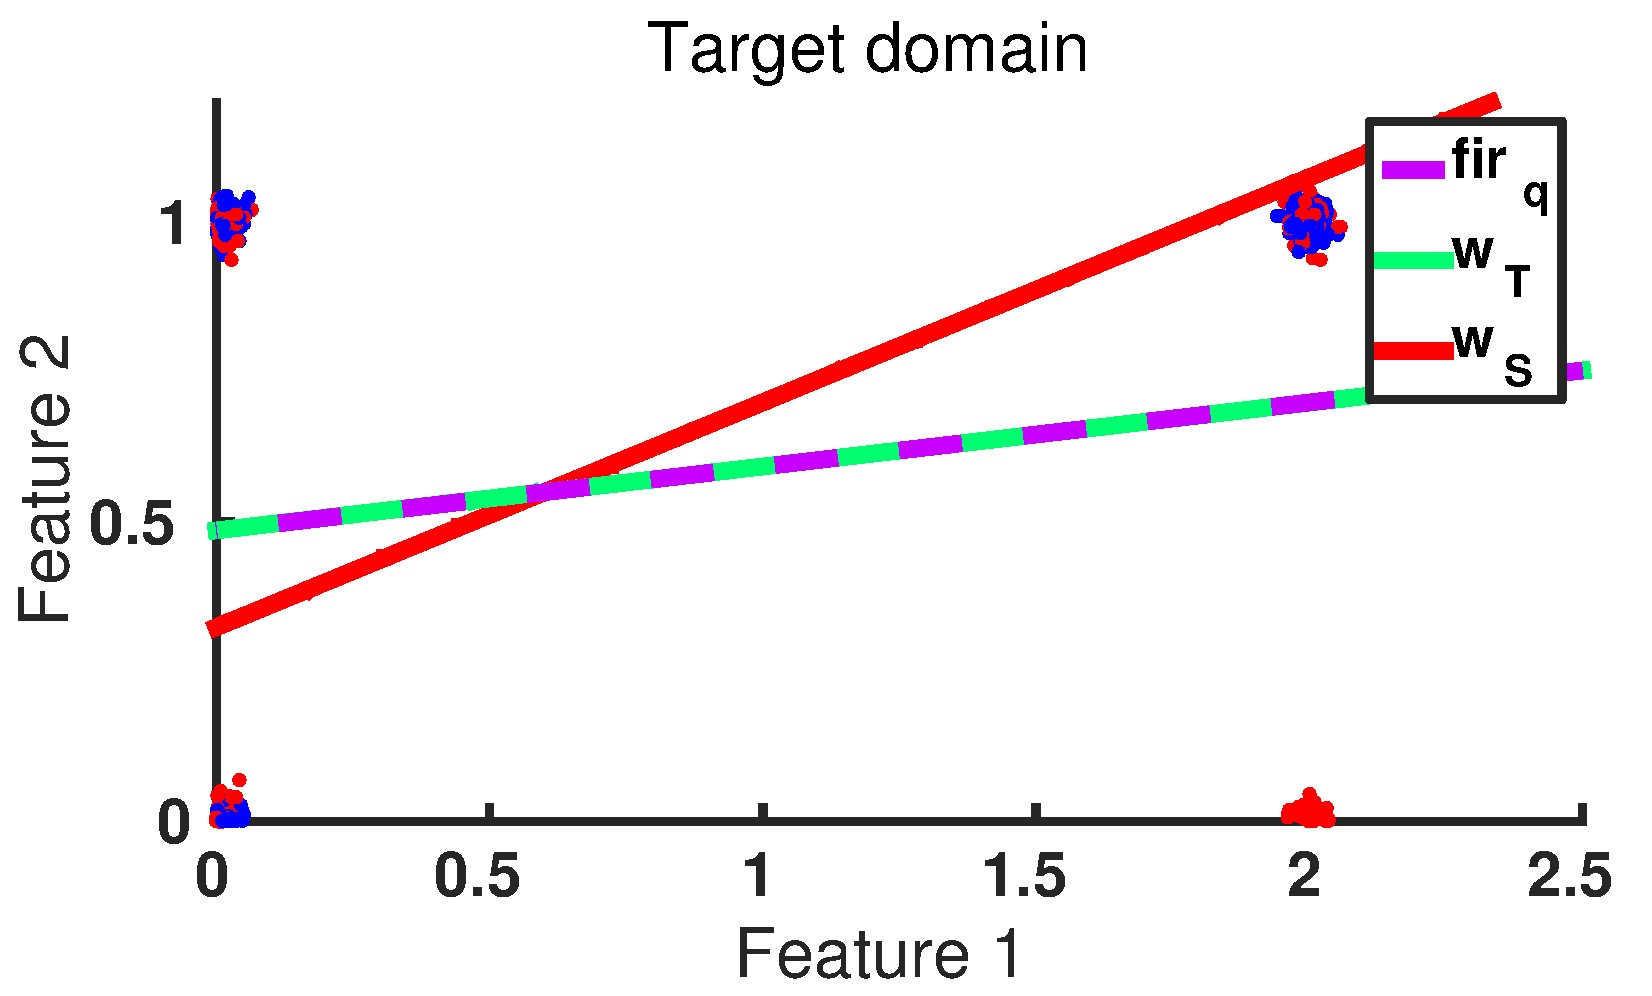
\includegraphics[width=.45\textwidth]{images/da_artexp_sens_model_convergence_Bern_square.eps} \hspace{5px}
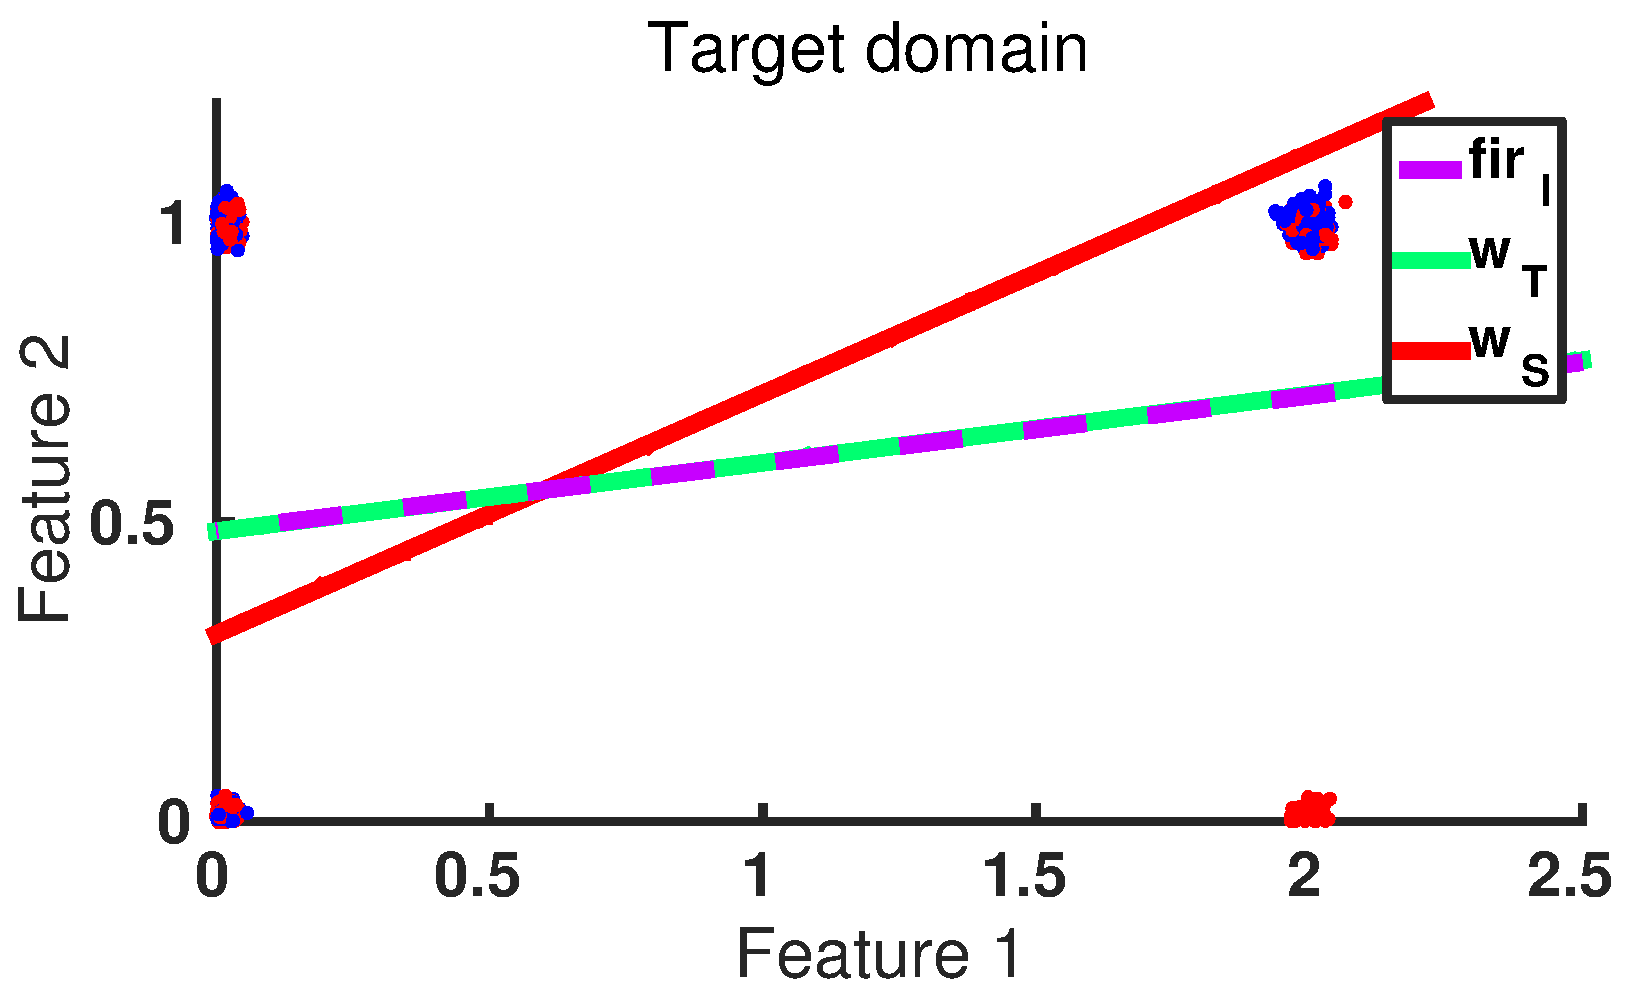
\includegraphics[width=.45\textwidth]{images/da_artexp_sens_model_convergence_Bern_log.eps}
\caption{The data is generated by Bernoulli class-conditional likelihoods and transformed using a Bernoulli transfer. Red and blue dots show different classes that have been jittered for visualization purposes. The lines are the decision boundaries found by the naive source classifier ($w_{S}$), the naive target classifier ($w_{T}$) and the adapted fir classifier ($fir$). Left shows the solutions of classifier with a quadratic loss and right with a logistic loss. Note that the adapted classifier finds the same boundary as the target classifier.}
\label{art1}
\end{figure}

Interestingly, if we generate datasets from different distributions and estimate the transfer parameters through dummy variables, the classifier also converges to the naive target classifier (see figure \ref{art2}). Successful adaptation does not depend on the data, but on our ability to estimate the appropriate transfer distribution. 

\begin{figure}[ht]
\centering
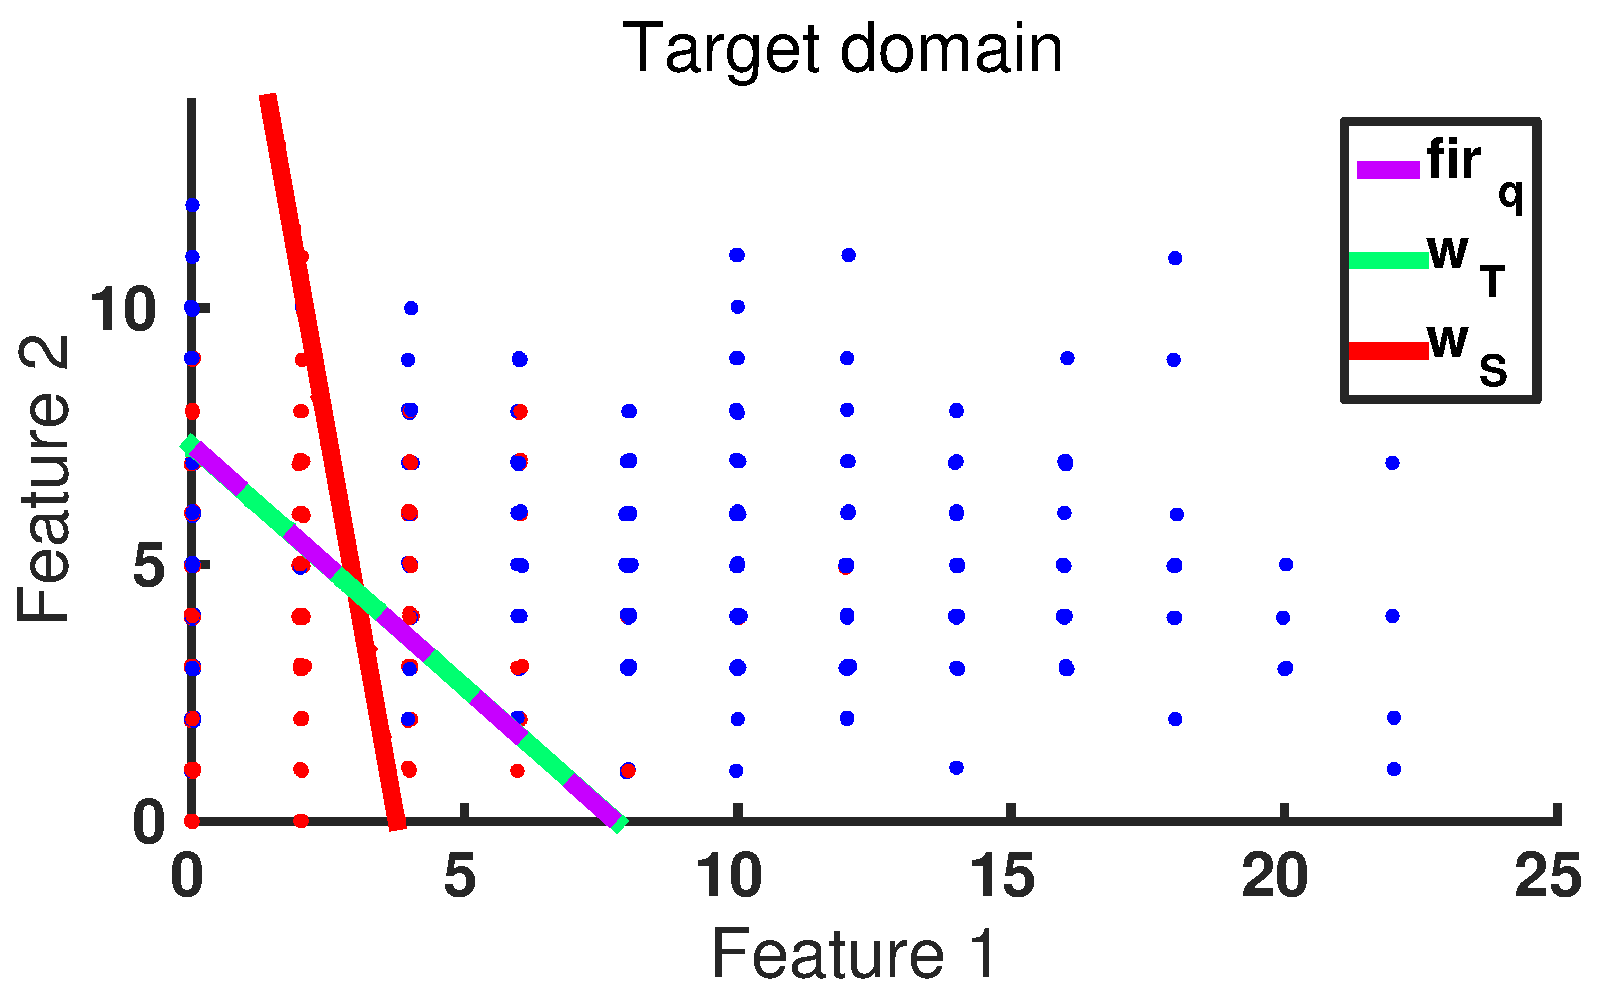
\includegraphics[width=.45\textwidth]{images/da_artexp_sens_model_convergence_Poisson_square.eps} \hspace{5px}
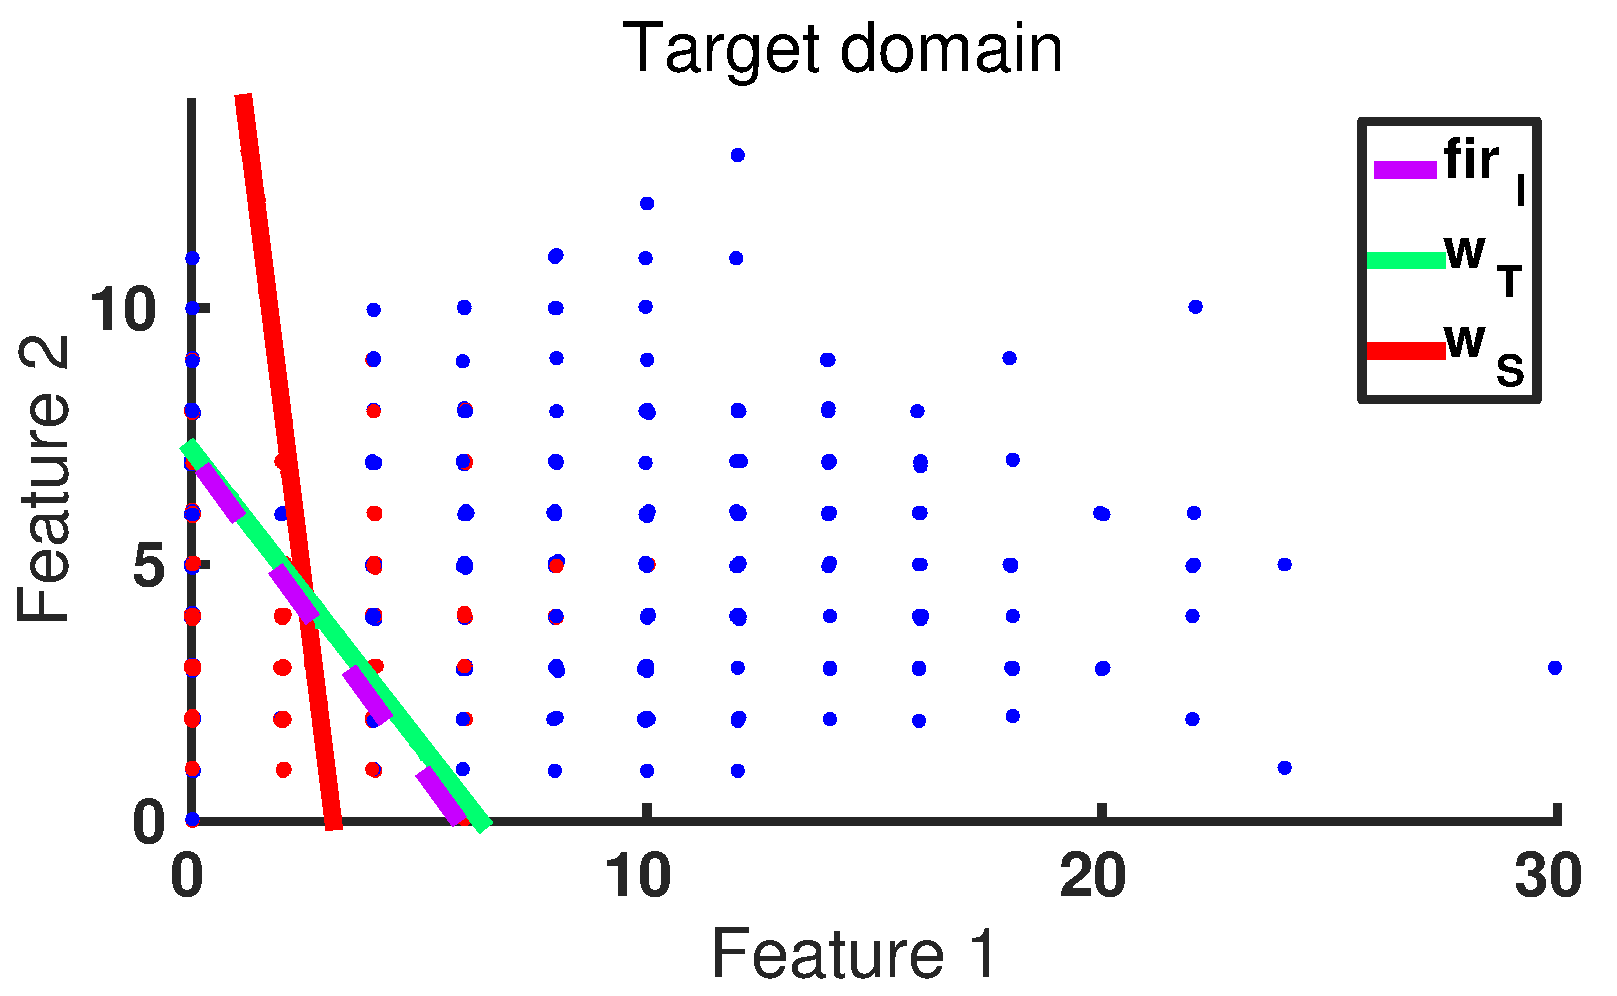
\includegraphics[width=.45\textwidth]{images/da_artexp_sens_model_convergence_Poisson_log.eps}
\caption{The plot shows a similar classification problem as figure \ref{art1}, but here the data was generated by Poisson distributions. Note that the regardless of the data, if there is a Bernoulli transfer our fir classifier can adapt to the target domain.}
\label{art2}
\end{figure}

\subsubsection{Learning curves}
If we plot the learning curves of our 3 classifiers, we can inspect how fast our adapted classifier converges to the target classifier. Figure (\ref{lc}) shows the mean classification error (lines) on an independent test set and standard deviation (shaded) of the source, target and adapted classifier. As expected the source classifier outperforms the target and adapted classifiers on the source domain (dotted lines), while the other two outperform the source classifier on the target domain (solid lines). To calculate the standard error of the mean, we took 30 repeats for every sample size. 

For a low-dimensional problem with no other domain dependencies than rate decreases, a few samples are enough to converge. Most likely, the number of samples needed will increase with the number of dimensions.

\begin{figure}[ht]
\centering
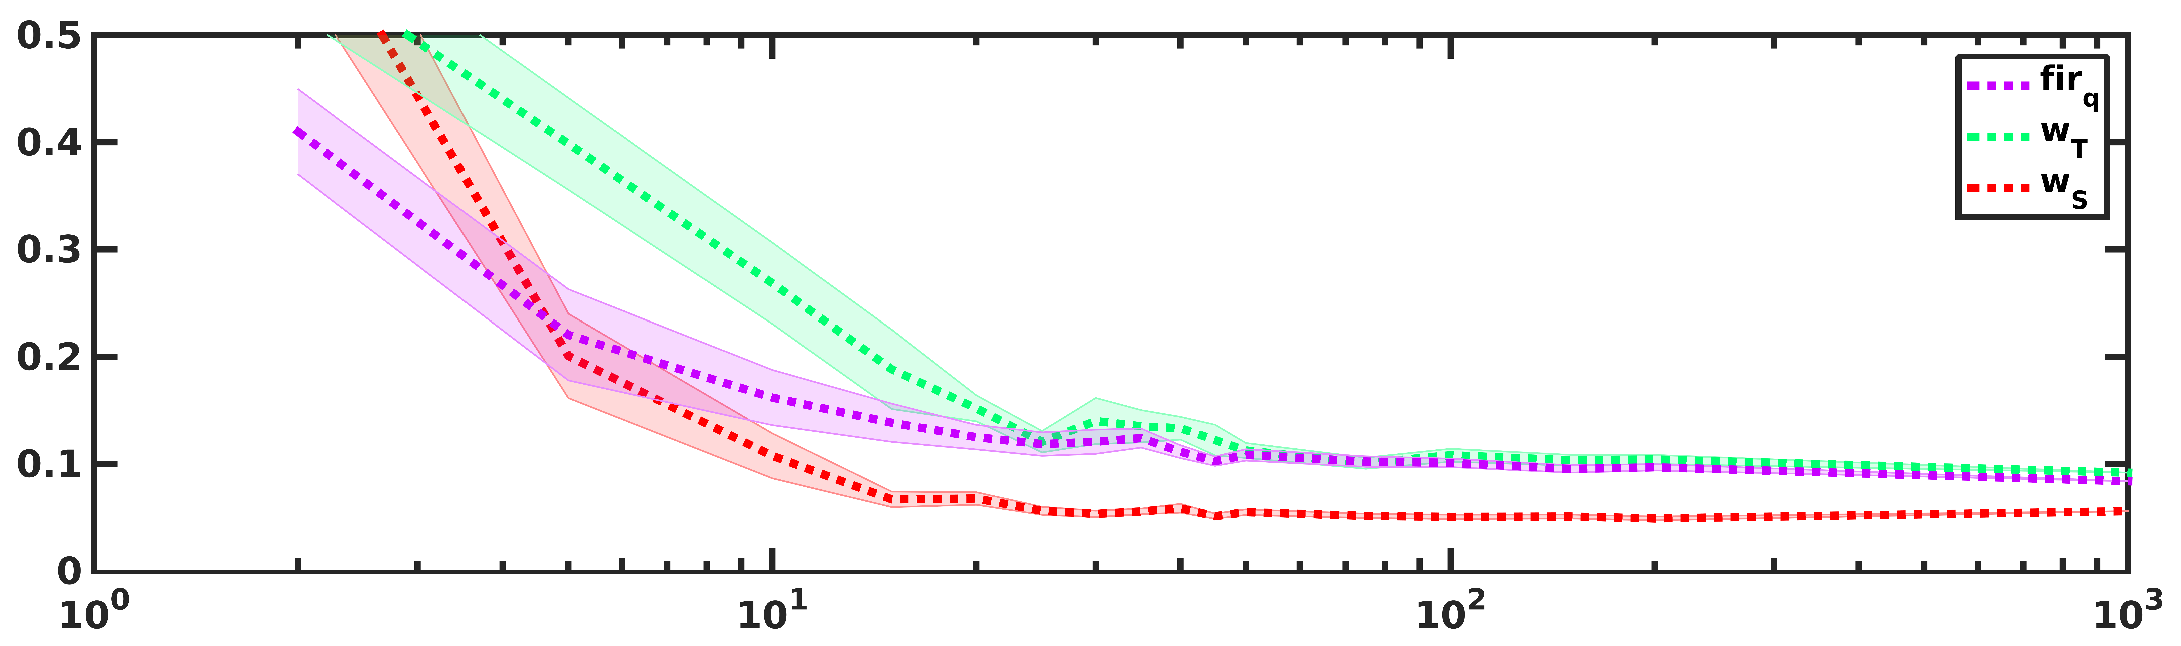
\includegraphics[width=1\textwidth]{images/learning_curveS.eps} \vspace{5px} \\
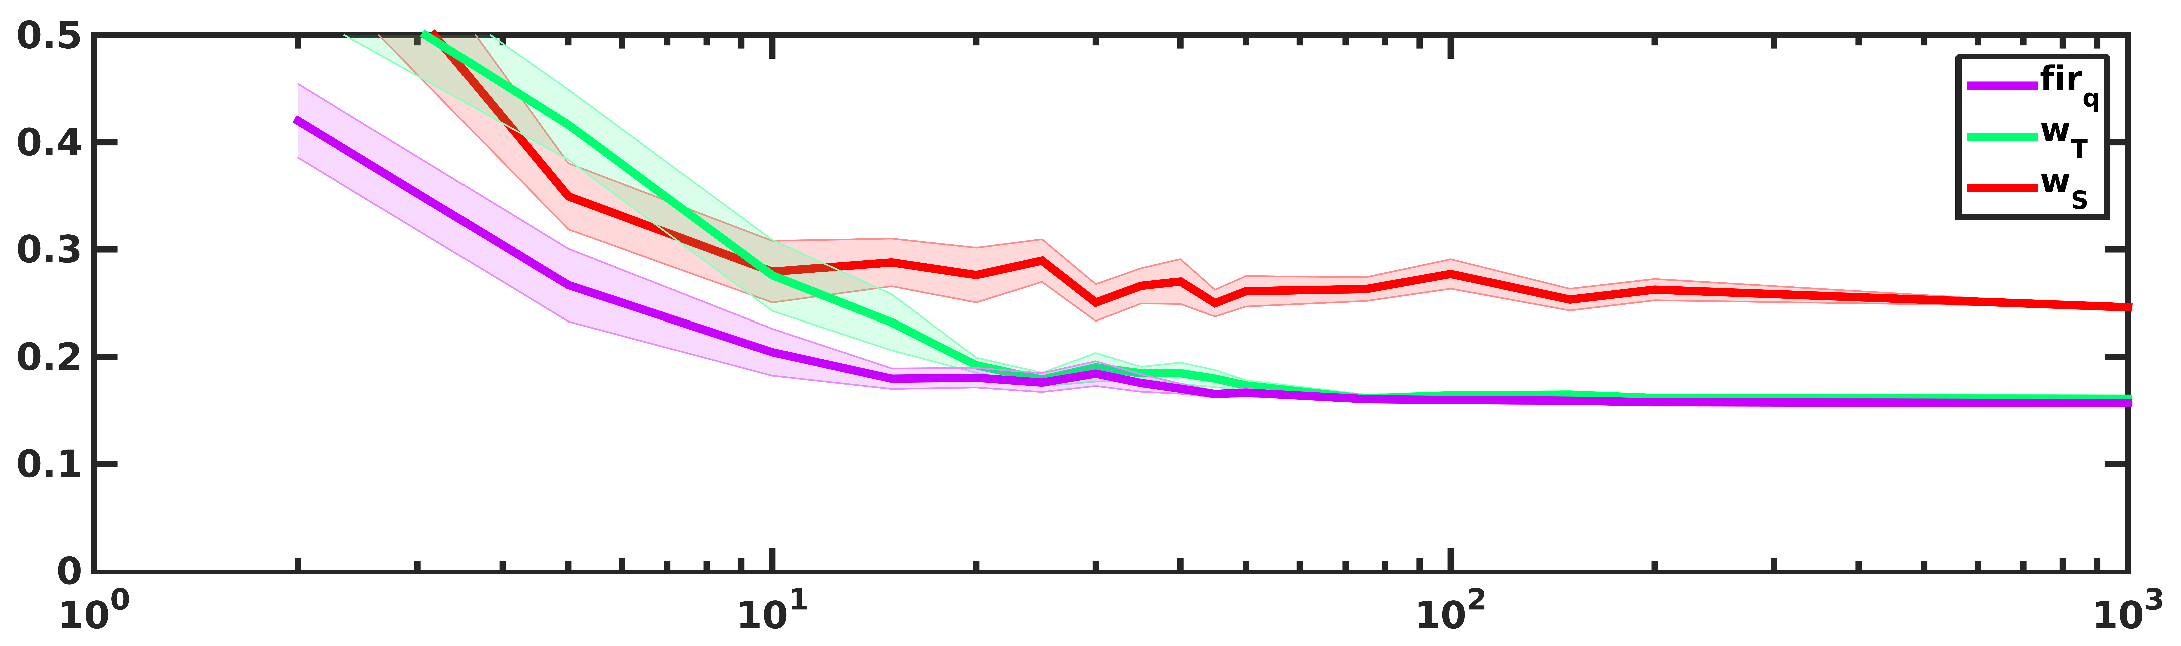
\includegraphics[width=1\textwidth]{images/learning_curveT.eps}
\caption{Learning curves of the source $w_{S}$, target $w_{T}$ and adapted classifier $fir_{qd}$. Left shows the error on an independent validation set generated from the same distributions as the source domain. Right shows the error on an independent validation set generated from the target domain.}
\label{lc}
\end{figure}

\subsubsection{Robustness to parameter estimation errors}
In this experiment, we study how fast classification error deteriorates as we increase the estimation error in the transfer parameters. Figure \ref{sens_params} shows an experiment where we added a value of 0, 0.1, 0.2 and 0.3 to the estimate the fir classifier made. Note that the classifier is quite robust to small errors but deteriorates for large errors.

\begin{figure}[ht]
	\centering
	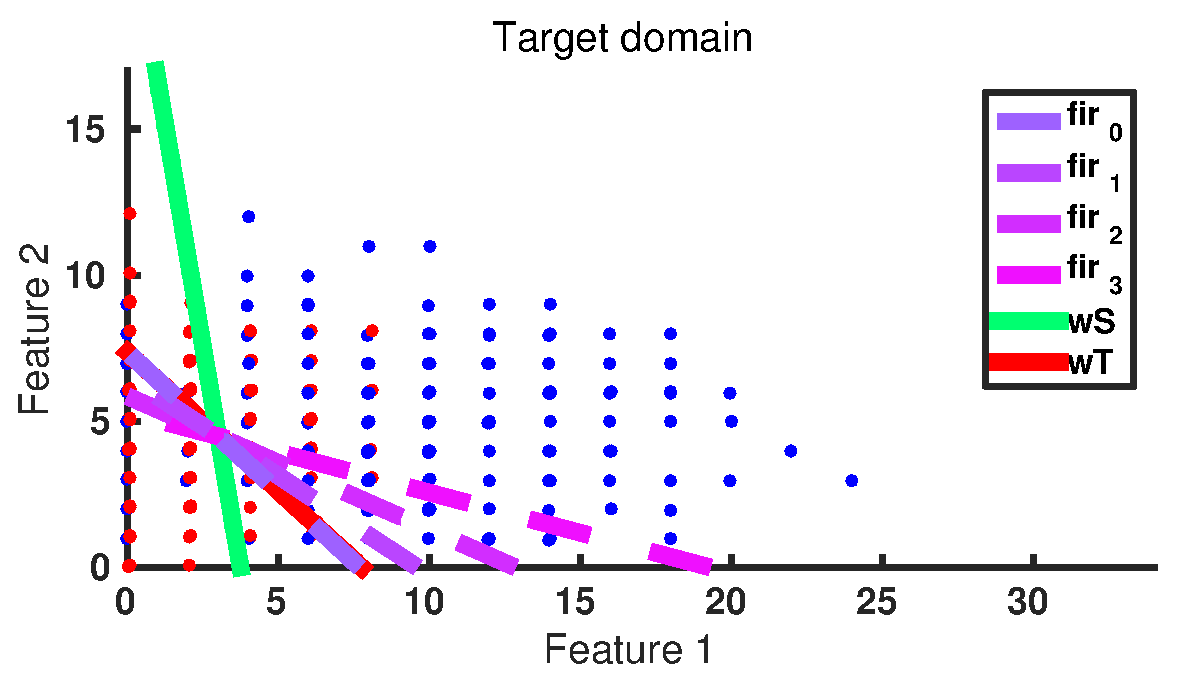
\includegraphics[width=.45\textwidth]{images/da_artexp_sens_params_square.eps} \hspace{5px}
	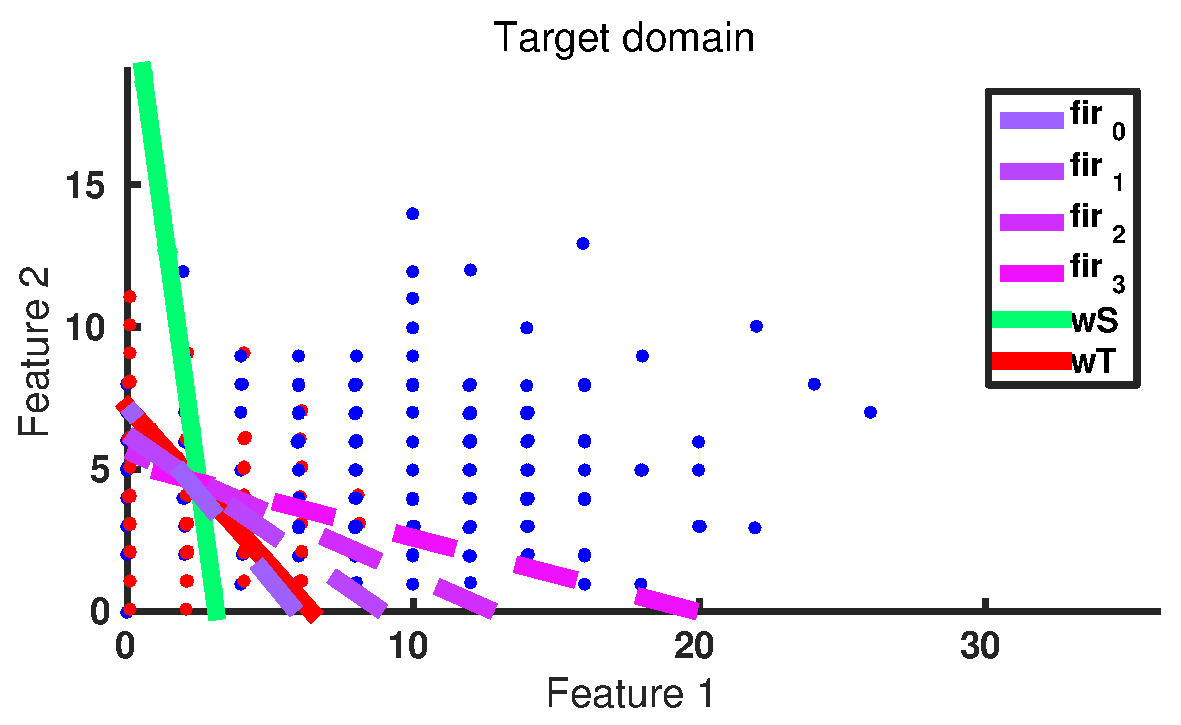
\includegraphics[width=.45\textwidth]{images/da_artexp_sens_params_log.eps} 
	\caption{Experiment to determine how sensitive the model is to errors in estimating the parameters of the transfer distribution. fir 0-3 shows the solution found by the adapted classifier for increments of 0, 0.1 0.2 and 0.3 to the transfer parameter estimate of feature 1. Left shows the quadratic loss and right shows the logistic loss.}
	\label{sens_params}
\end{figure}

\subsection{Natural datasets}
We have selected a number of domain adaptation problems consisting of nonnegative integer data, either in a (visual) bag-of-words representation or pixel intensities (between 0 and 255). They are typical scenarios where we believe a dropout or blankout transfer occurs. Three are three natural language based and two are based on images.

We compare our fir classifier with 3 competing methods, two based on instance reweighting and one based on a domain-invariant subspace. To faciliate a fair evaluation of the adaption method, we train all methods using the same loss function. This is to ensure that performance measures do not depend on the classifier's flexibility or complexity. In order to compare the performance of an adapted classifier, we train and test classifiers on the same domain as well. The error rates for within-domain combinations can be considered the target classifiers and would represent the best performance the adapted classifier should be able to obtain.

%For the subspace alignment (sa) method, the number of eigenvectors we keep is 100. The choice of the size of the subspace is important, but since the eigenvalue decomposition is computationally very expensive for high-dimensional datasets, we feel this is a fair parameter choice. 
For structural correspondence learning (scl), we took the 30 most frequent features as pivots and learned to predict their outcomes based on the whole using a modified Huber Loss. The subspace then consists of finding the eigenvectors of the pivot predictors. in our standard instance reweighting method (irw) we estimated the weights for each sample by computing the posterior probability of belonging to one domain using a logistic classifer. For kernel mean matching (kmm), we used a radial basis function kernel. 

\subsubsection{Crossvalidation}
The goal of the classifier is to predict labels of new samples and to get a measure of generalization, we perform 3 repeats of 3-fold crossvalidation. However, crossvalidation becomes tricky for transfer learning. If we split the training dataset in folds, we obtain a classifier that generalizes better to unseen source samples. However, that is not what we are interested in. The goal is to generalize better to unseen target samples. Therefore, we split the target data in folds where we hold out 1 fold for validation and use the remaining folds for estimating the transfer parameters. 

\subsubsection{Amazon}
The amazon sentiment analysis dataset is a popular domain adaptation set and consists of Amazon's written product reviews, first used in \cite{blitzer2007biographies}. The data is a 30 000 words bag-of-words representation of a 27677 reviews with the product categories as the domains; books, dvds, electronics and kitchen appliances. The label is derived from the binarized 5-star rating. The number of reviews per domain is fairly balanced, as are the classes. There are clear differences in how often words are used across domains. Figure \ref{eg_amazon} shows the normalized frequencies of some example words. 

\begin{figure}[ht]
\centering
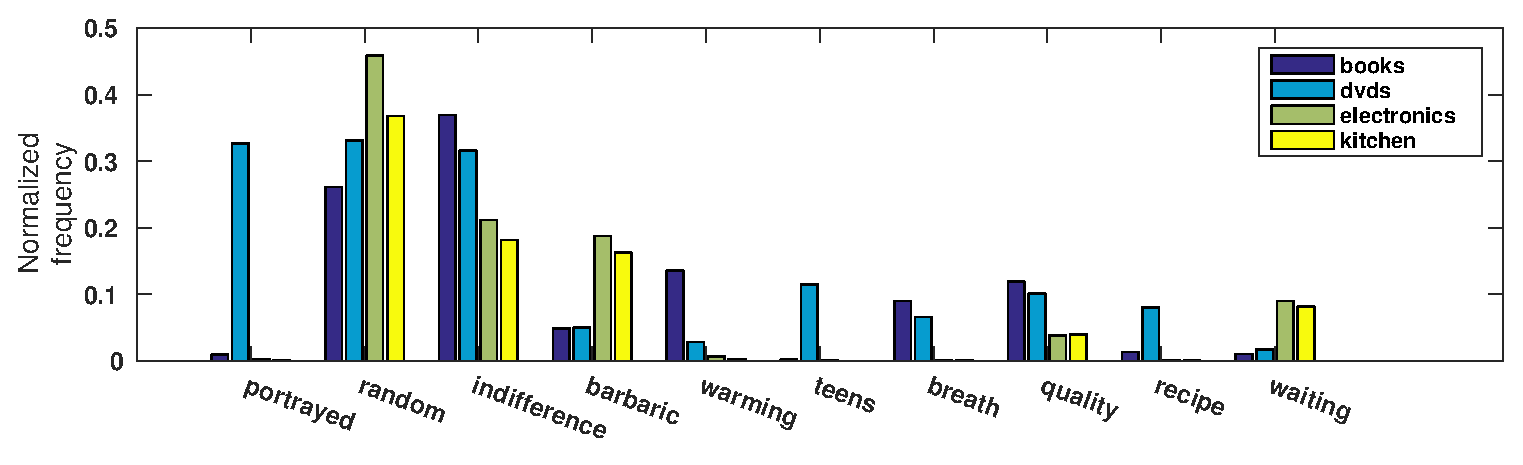
\includegraphics[width=\textwidth]{images/eg_amazon.eps}
\caption{Normalized frequencies across domains of some example words of the amazon dataset. Note that some words can be quite common in one domain, but virtually absent in another.}
\label{eg_amazon}
\end{figure}

In figure \ref{err_amazon} we report the mean misclassification error and standard errors of the logistic loss classifiers on all pairwise combinations of domains. The results indicate that none of the classifiers consistently outperforms the other ones. There are also few combinations where the adapted classifiers outperform the naive one, indicating that there are complex dependencies between these domains.

\begin{figure}[ht]
	\centering
	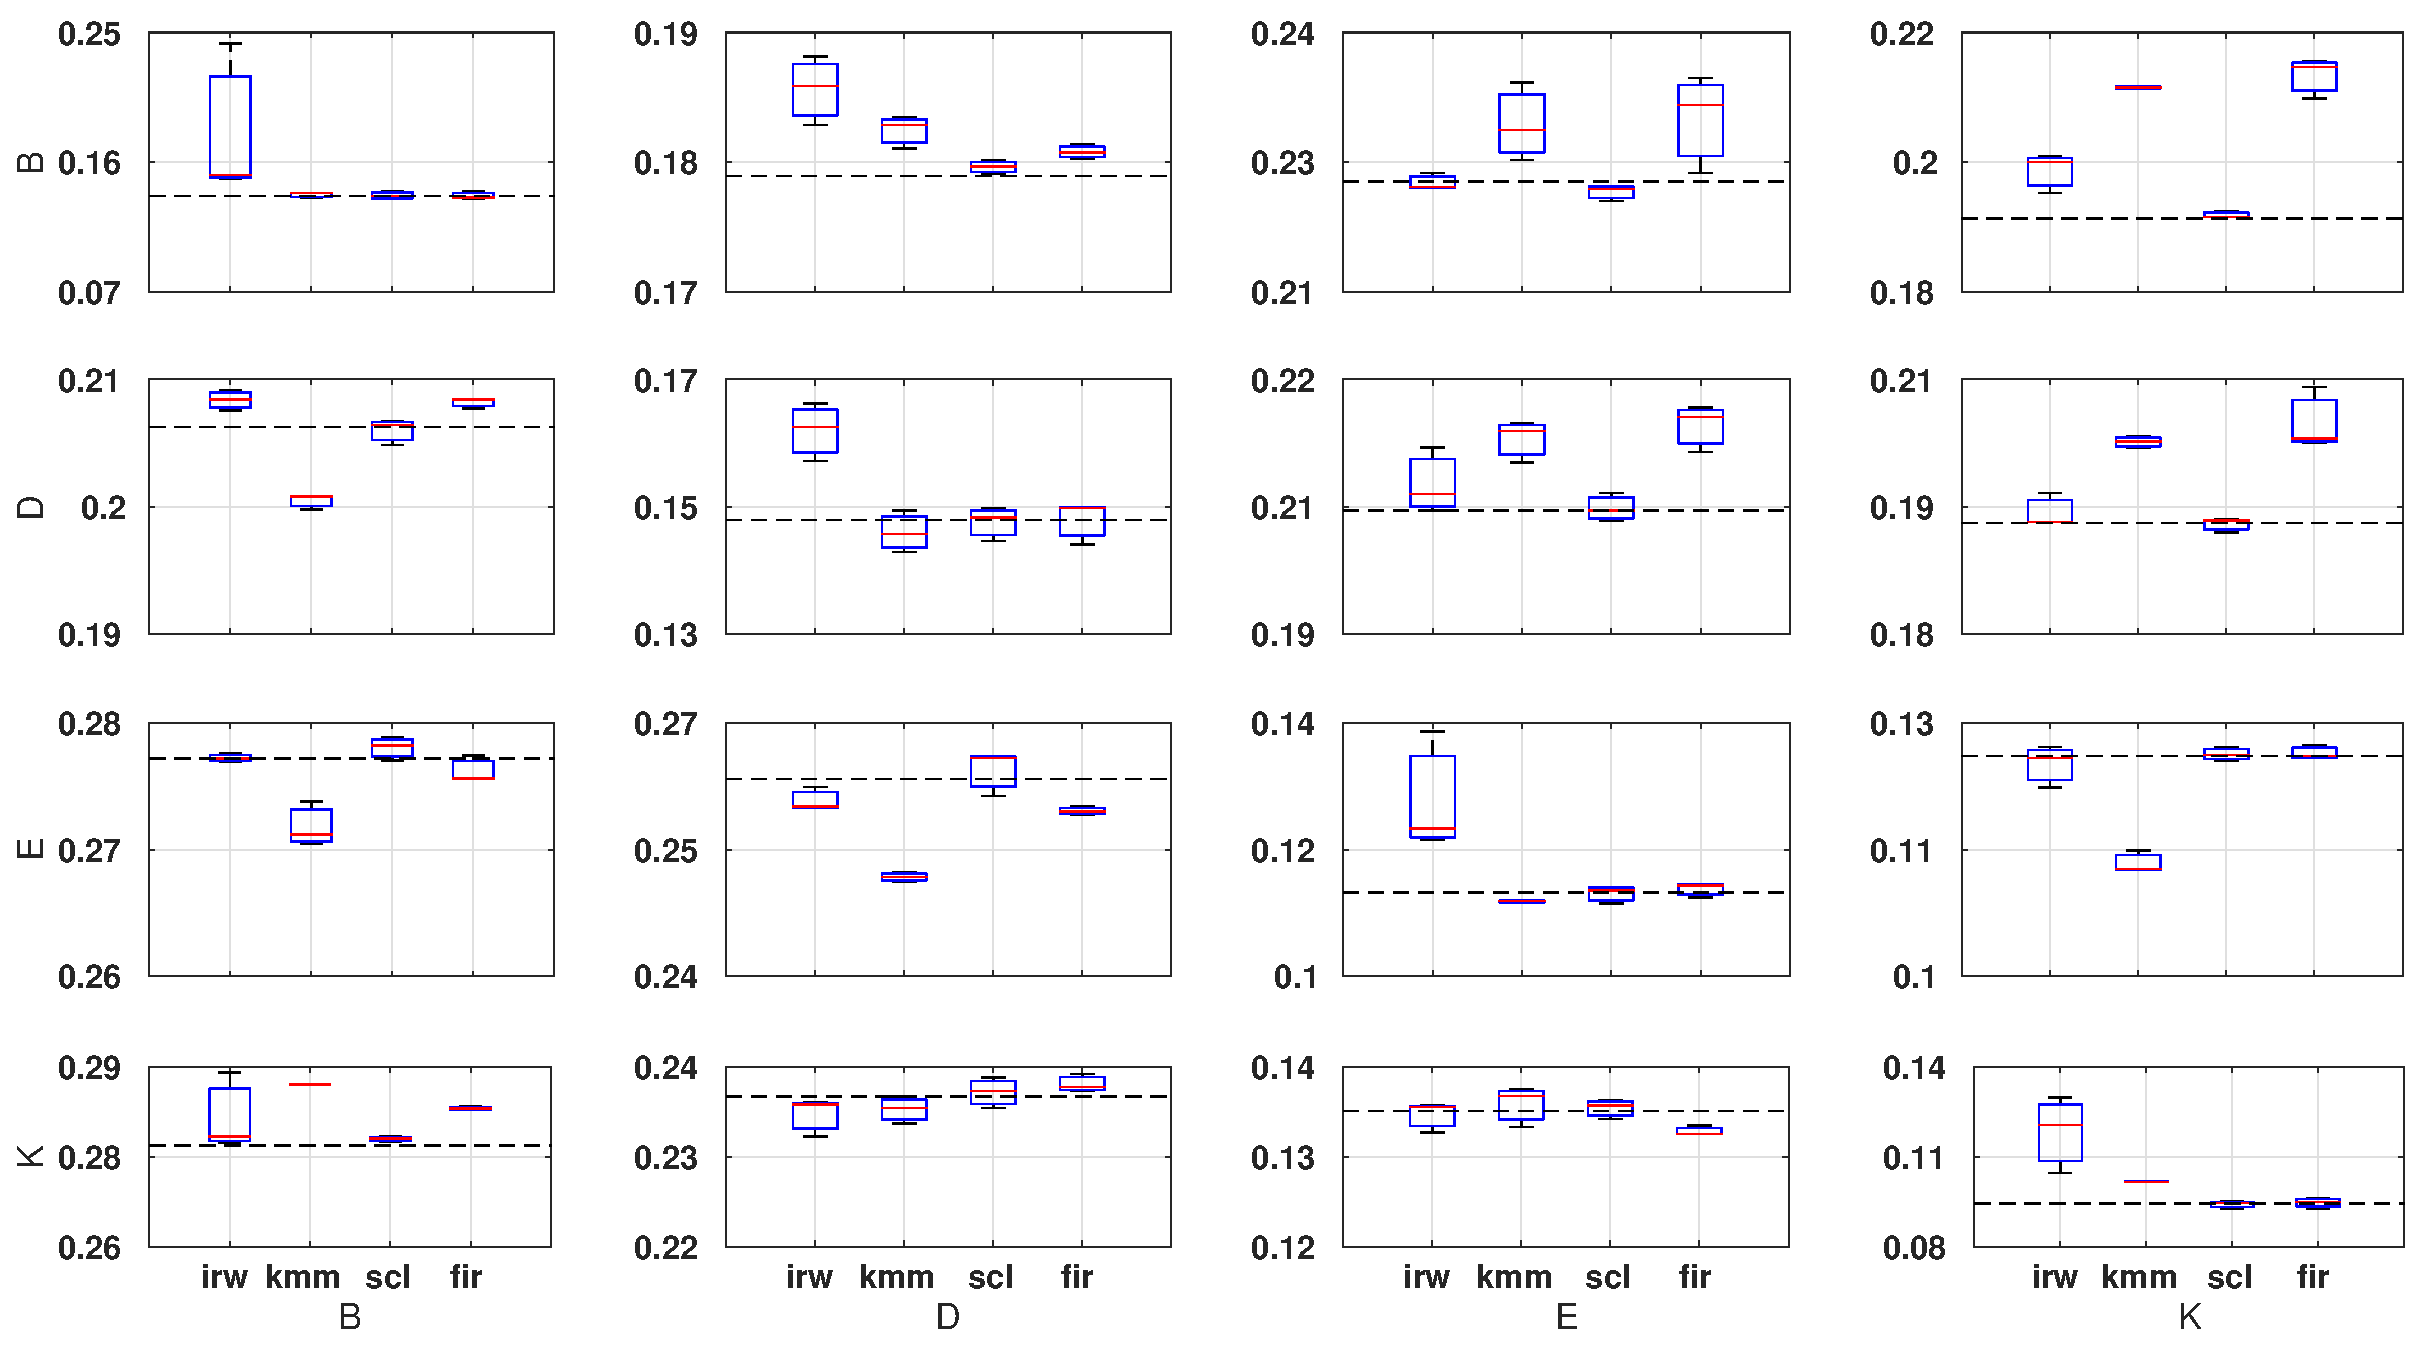
\includegraphics[width=1\textwidth]{images/err_amazon_box.eps} 	
	\caption{Box plots of the mean classification error of the repeats of the crossvalidation procedure. The dotted black line is the mean classification error of a naive logistic regressor. Grid shows pairwise combinations of traning on one source domain (rows) and testing on a target domain (columns). B = 'books', D = 'dvd', E = 'electronics' and K = 'kitchen'.}
	\label{err_amazon}
\end{figure}


\subsubsection{IMDB}
The IMDB movie database is provided by \cite{maas2011learning} and contains written reviews of movies labeled with a 1-10 star rating. We binarized the labels as $>$ 5 postive and $\leq$ 5 as negative, leaving us with nicely balanced classes. In order to create a domain adaptation dataset, we assigned a genre to each review based on the dominant genre of the corresponding movie. Since some movies have multiple genres, there is prior knowledge that the domains are dependent. However, the genres are so unbalanced that we decided to keep only the movies related to the three most common genres; action, family or war. For computational reasons we only kept features that had more than 100 counts in total, leaving us with 4180 features for 21954 samples.
					
\begin{figure}[ht]
\centering
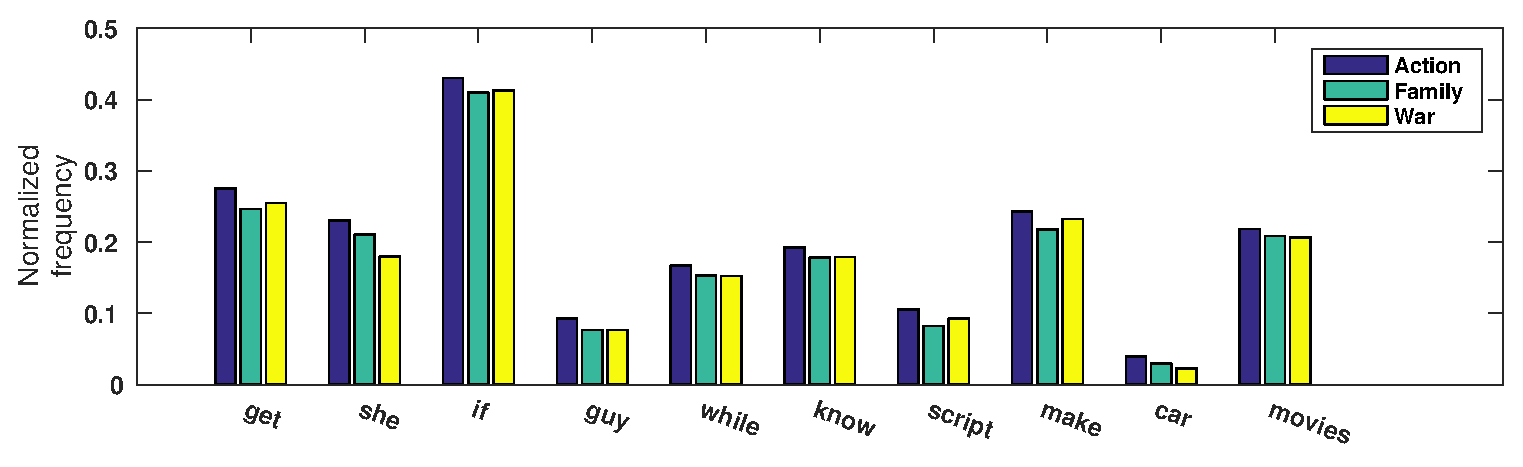
\includegraphics[width=\textwidth]{images/eg_imdb.eps}
\caption{Normalized frequencies across domains of some example words of the imdb dataset. Note that the frequencies are more similar across domains than for the amazon dataset.}
\label{eg_imdb}
\end{figure}

The normalized frequencies of this dataset show few differences across domains (see figure \ref{eg_imdb}). That would explain why for this dataset, there are also small differences between the error rates of the within-domain combinations versus the between-domain combinations. Figure \ref{err_imdb} indicates that there is again no clear consistently better classifier. In some combinations, a form of instance reweighting leads to a significantly better classifier, but for other combinations it leads to worse combinations.
																
\begin{figure}[ht]
	\centering
	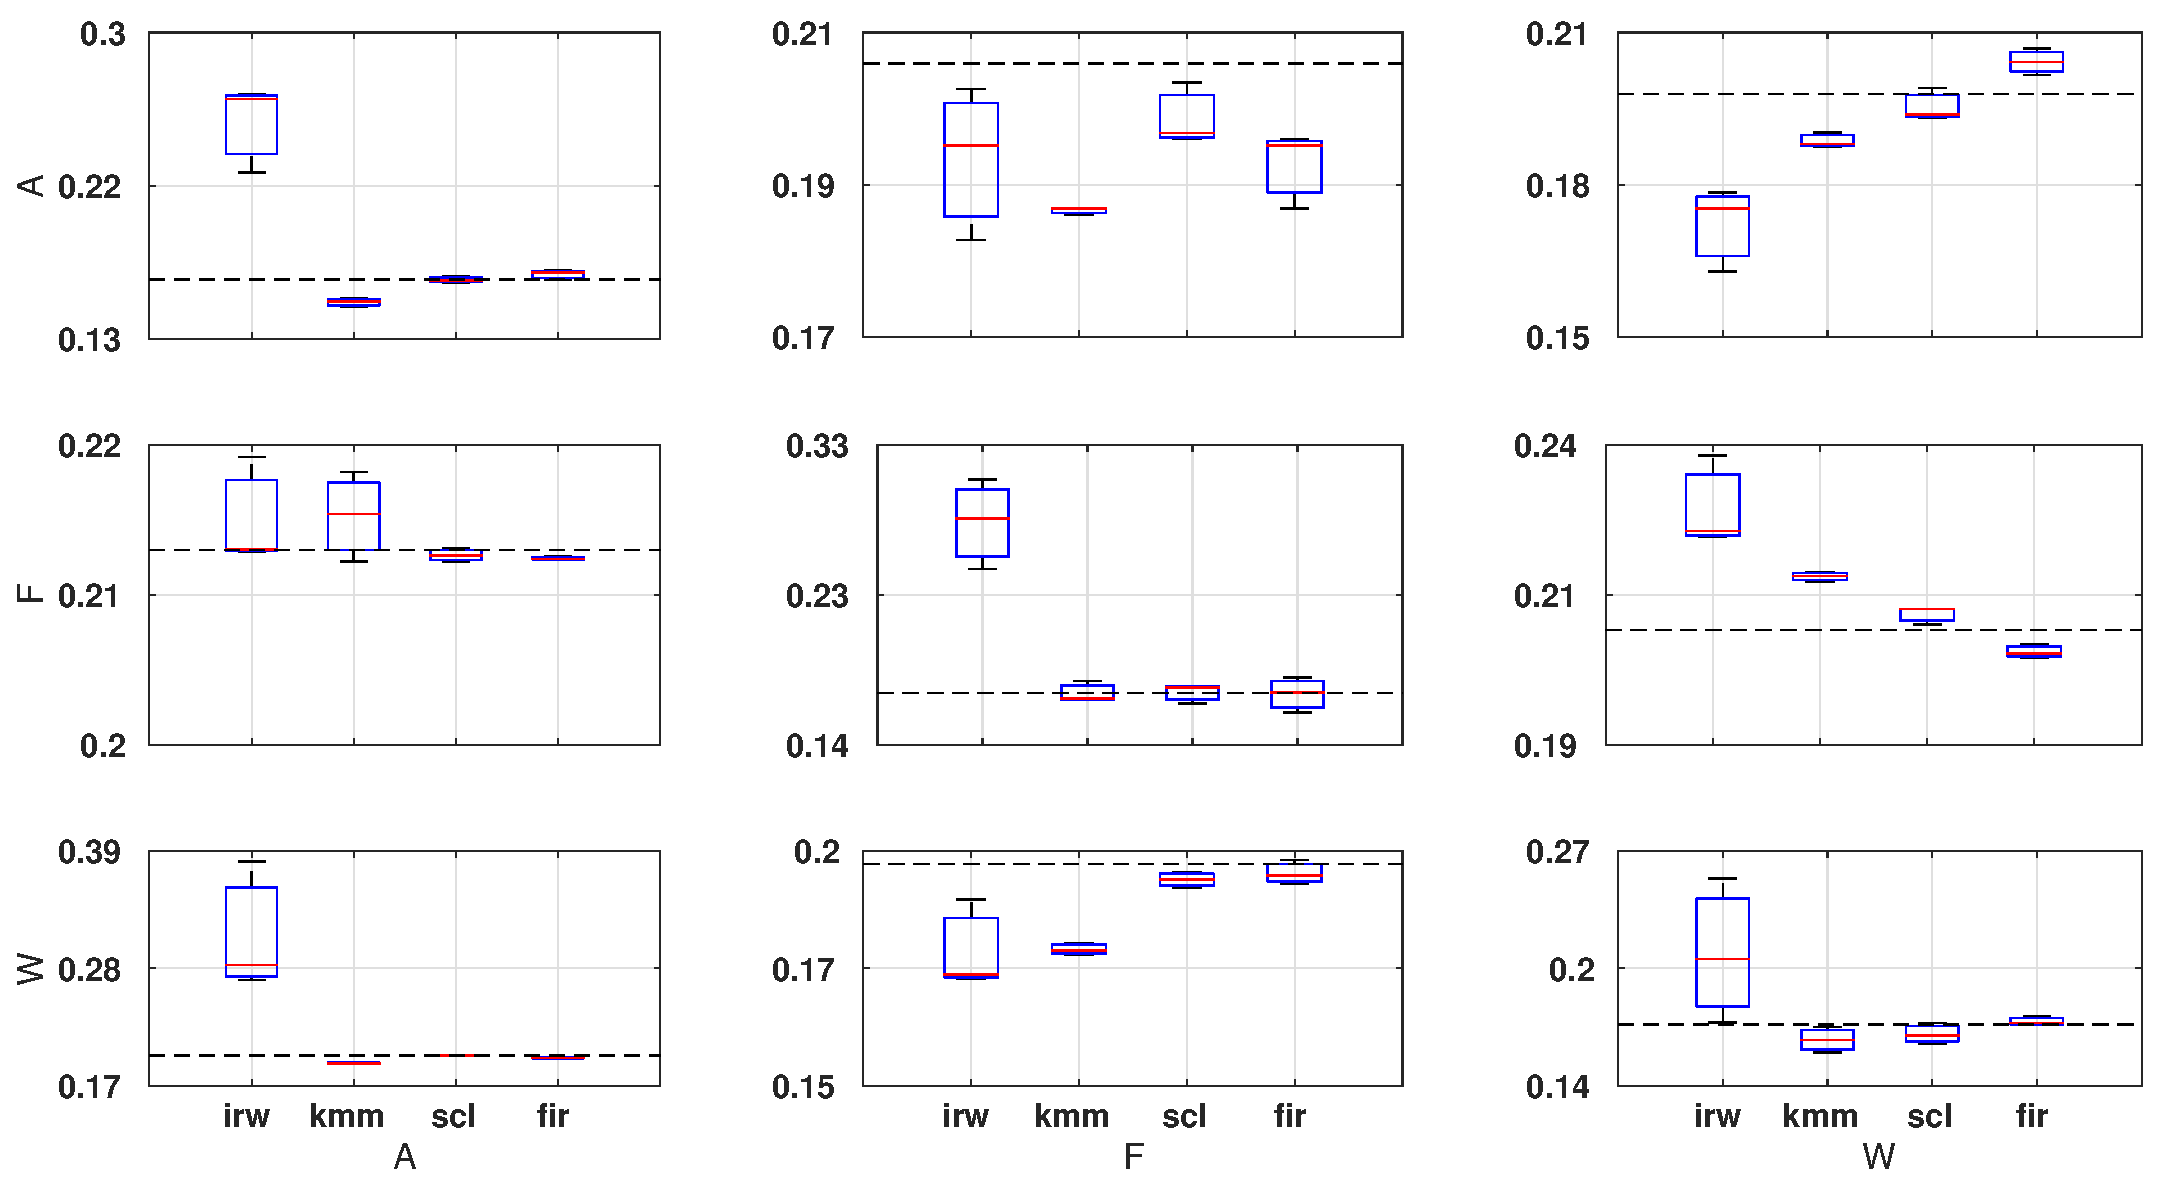
\includegraphics[width=\textwidth]{images/err_imdb_box.eps}
	\caption{Box plots of the mean classification error of the repeats of the crossvalidation procedure. The dotted black line is the mean classification error of a naive logistic regressor. Grid shows pairwise combinations of traning on one source domain (rows) and testing on a target domain (columns). A= 'action', F = 'family' and W = 'war'.}
	\label{err_imdb}
\end{figure}


\subsubsection{Spam}
We can also view spam detection in different media as a domain adaptation problem. Here we have collected two datasets from the UCI machine learning repository, one containing the enron e-mail spam database and one containing the sms-spam dataset. It would be interesting to see if we can pick out spam text messages based on an e-mail spamfilter or vice versa. Both datasets were parsed into a bag-of-words representation but we kept only the 4272 words that occurred in both domains as the new common feature space. Classes are balanced but the domains are very imbalanced; 5000 out of 40 000 documents are text messages.

\begin{figure}[ht]
	\centering
	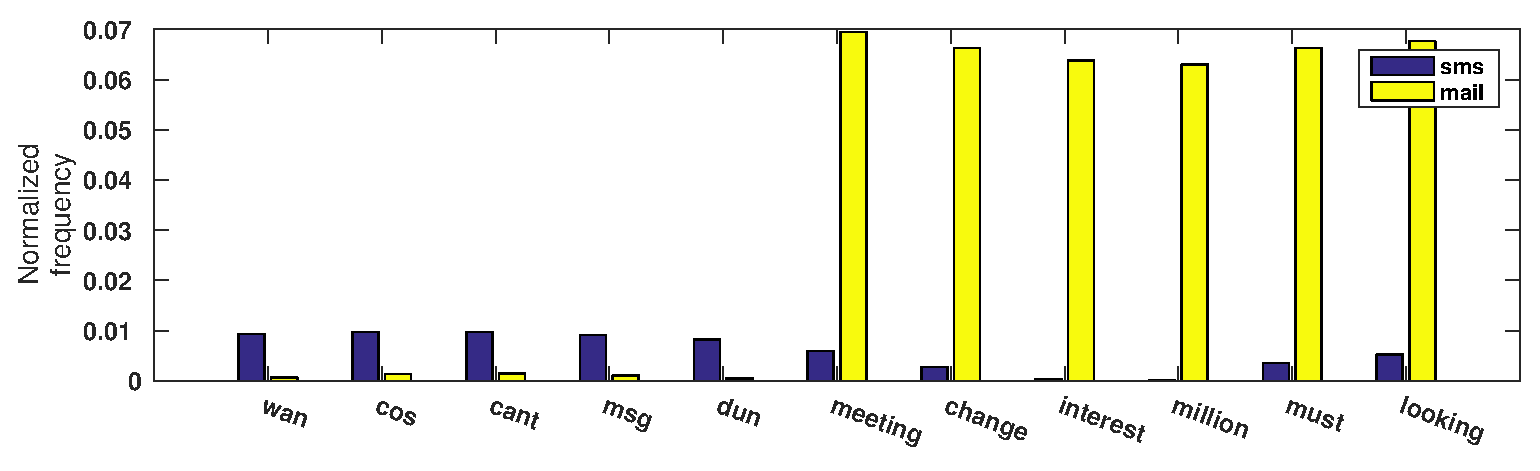
\includegraphics[width=1\textwidth]{images/eg_spam.eps}
	\caption{Normalized frequencies across domains of some example words of the imdb dataset. Note that the frequencies and word types are very different for the domains.}
	\label{eg_spam}
\end{figure}

Figure \ref{eg_spam} is a good example of the differences between the two domains. Text messages use shortened words and do not have very common phrases, while email messages are more formal and tend to use the same kinds of words. It tells us that these domains are extremely different. If we study figure \ref{err_spam} we can see that the error is low within domains. Because we are using linear classifiers, we can conclude that the domains are almost linearly separable. If we study the between-domain errors, we see that it rapidly falls back to chance. This is very interesting finding; apparently the domains are so dissimilar that few to none of the discriminative features in the source domain are discriminative in the target domain. 

\begin{figure}[ht]
	\centering
	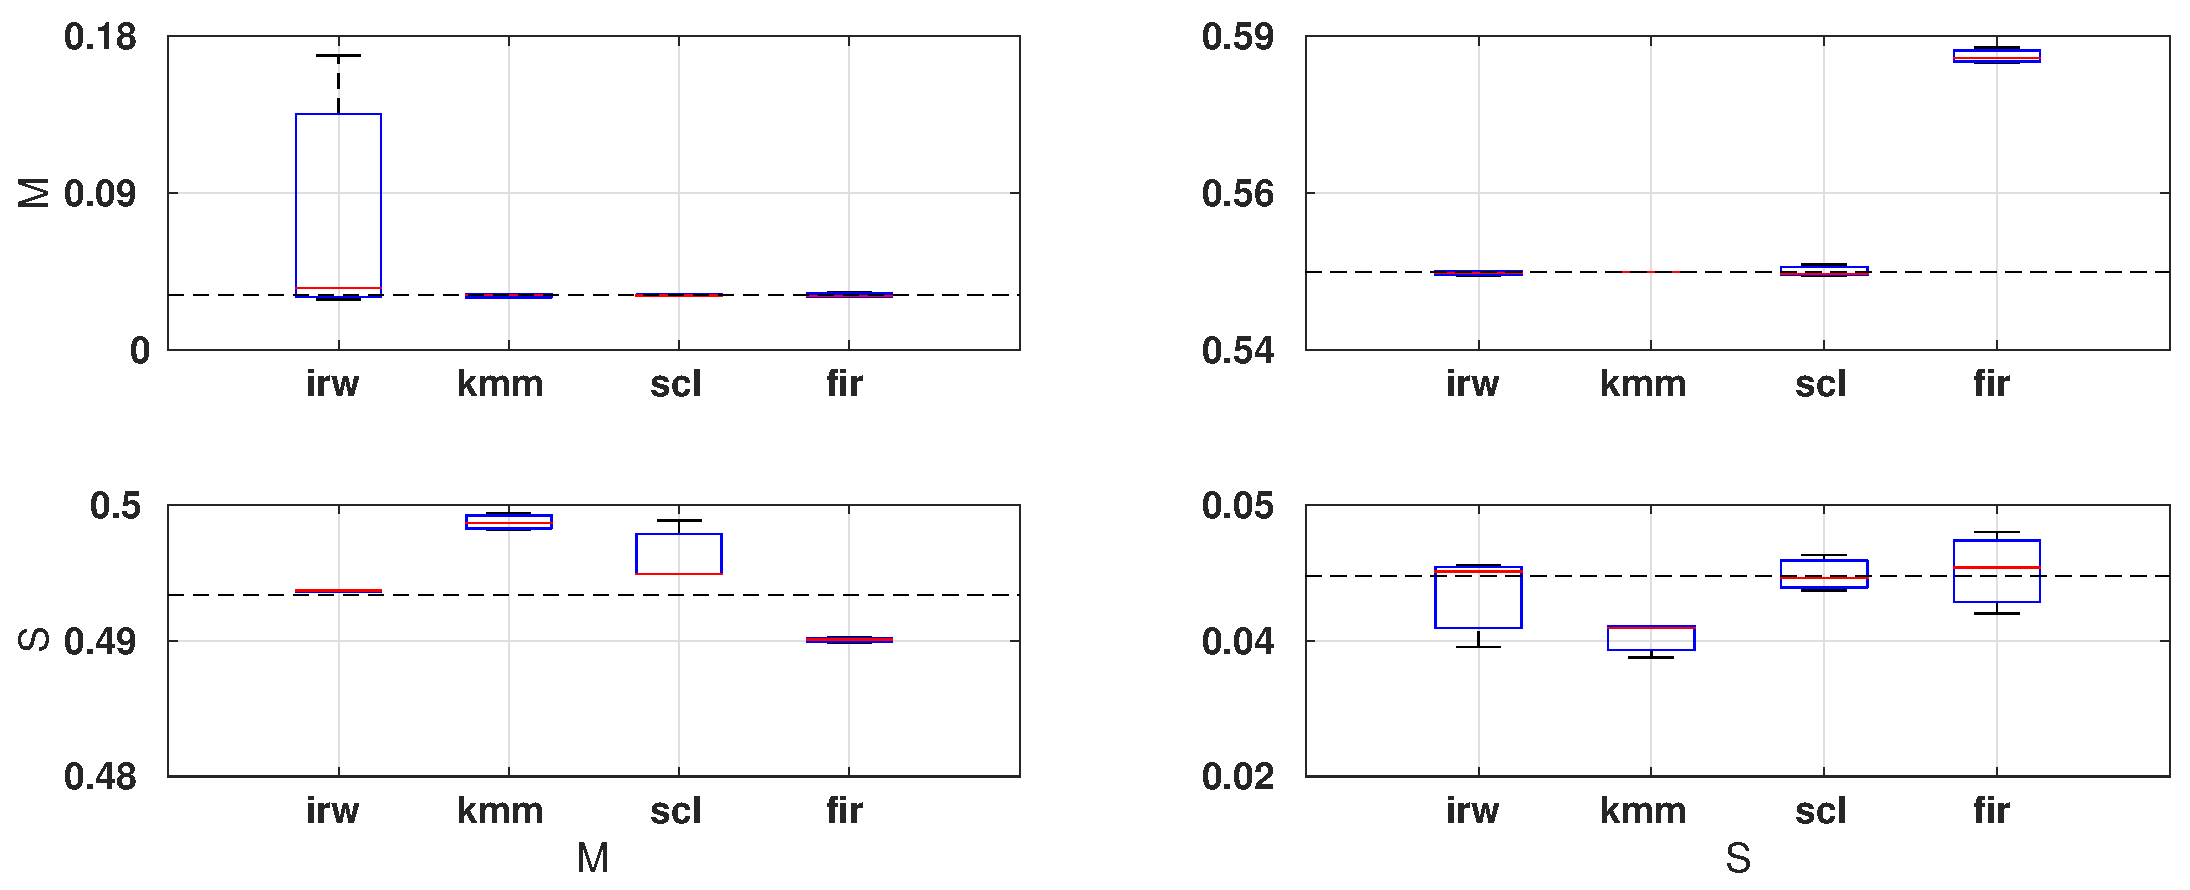
\includegraphics[width=1\textwidth]{images/err_spam_box.eps}
	\caption{Box plots of the mean classification error of every repeat of the crossvalidation procedure. The dotted black line is the mean classification error of a naive logistic regressor. Grid shows pairwise combinations of traning on one source domain (rows) and testing on a target domain (columns). S = sms' and M = 'mail'.}
	\label{err_spam}
\end{figure}

\subsubsection{Digits}
For this image dataset, we gathered 3 different versions of recorded handwritten digits from the UCI machine learning repository. The first is the well known MNIST dataset, the second the SEMEION set and the third the USPS set. All images are downsampled to 16 by 16 pixels, examples are show in figure \ref{eg_digits}. Again the classes are fairly balanced, but the domains are not: we took 60 000 images of MNIST, ~1500 from SEMEION and ~9000 from USPS. 

\begin{figure}[ht]
	\centering
	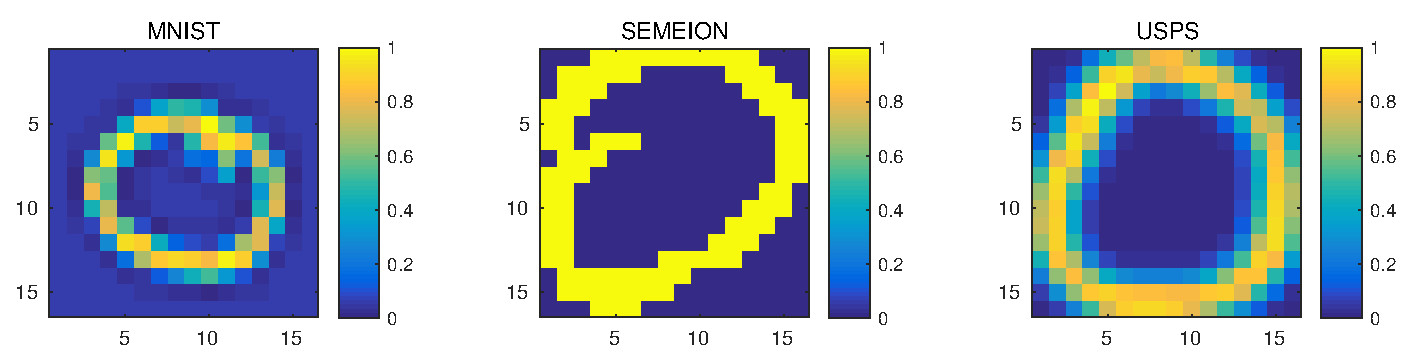
\includegraphics[width=1\textwidth]{images/digits_examples.eps}
	\caption{Examples of handwritten digits in each domain}
	\label{eg_digits}
\end{figure}

Figure \ref{err_digits} tells us that some combinations of data lead to poor adaptation while others can have a tremendous improvement. If we inspect some of the examples from each domain (see figure \ref{eg_digits}), we can see that USPS uses the outer features more than the other domains. Since we are only able to adapt to features that are used less frequently, and not more frequently, going from the denser domain to the sparser domain will lead to improvements. 

For this dataset, our fir classifier seems to be consistently outperforming the other methods. This could be due to the fact that the other methods were specifically built for text data while our method is more general.

\begin{figure}[ht]
	\centering
	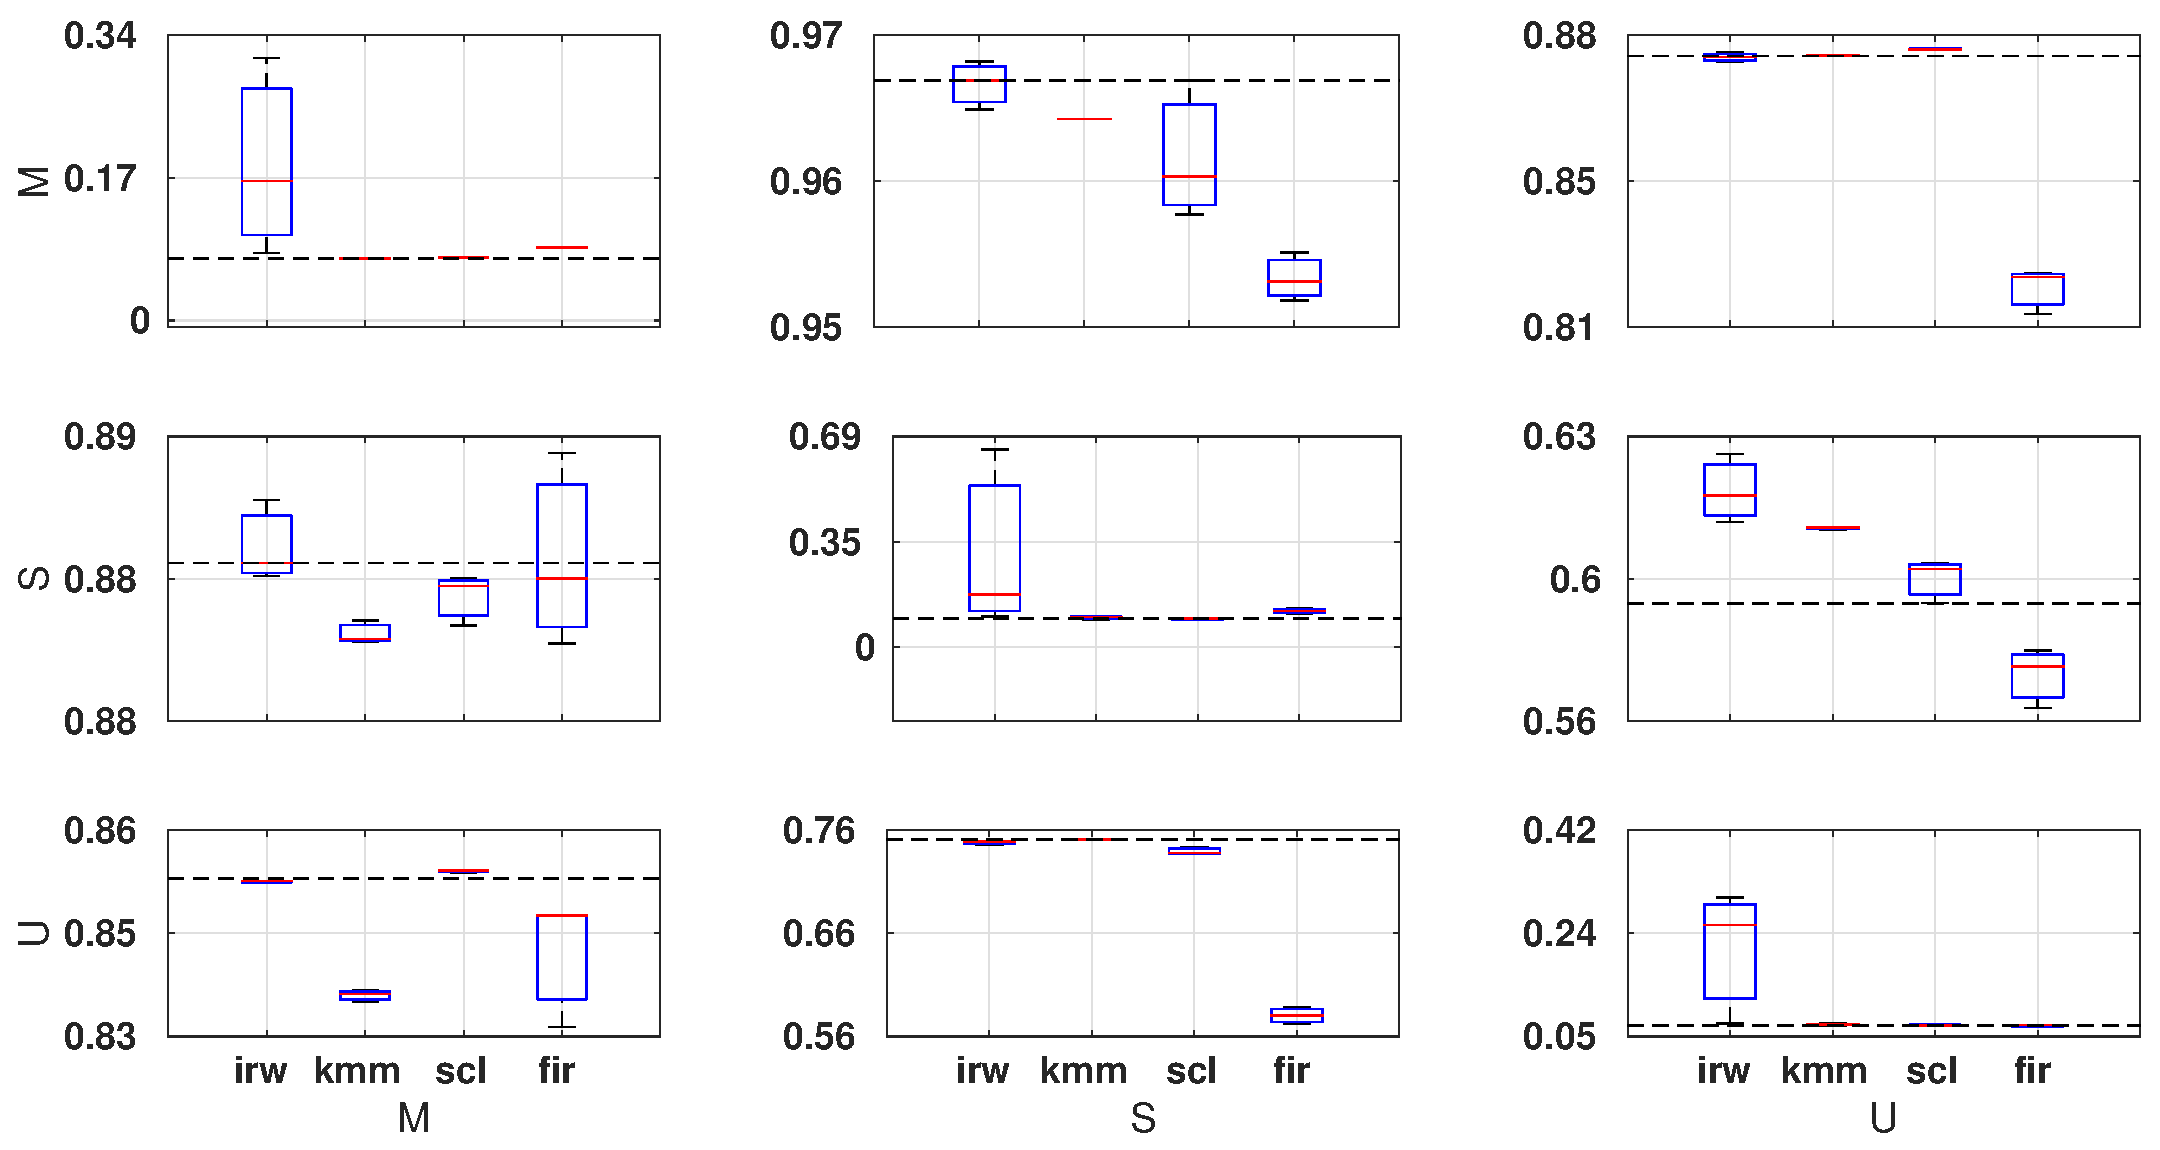
\includegraphics[width=1\textwidth]{images/err_digits_box.eps}
	\caption{Box plots of the mean classification error of every repeat of the crossvalidation procedure. The dotted black line is the mean classification error of a naive logistic regressor. Grid shows pairwise combinations of traning on one source domain (rows) and testing on a target domain (columns). M='mnist', S='semeion' and U='usps'.}
	\label{err_digits}
\end{figure}

In this case, it is also interesting to visualize the transfer parameters. Figure \ref{eg_digits2} (middle) shows the parameters with left the weights of a naive classifier and right the adapted classifier. Note that the new weights have been regularized more strongly in pixels with high transfer parameters.

\begin{figure}[ht]
	\centering
	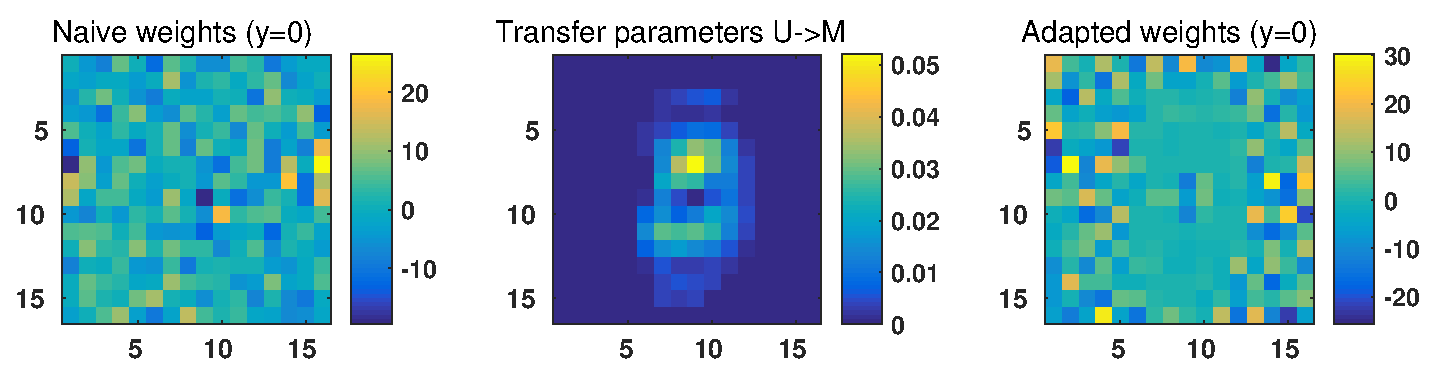
\includegraphics[width=1\textwidth]{images/tf_digits.eps}
	\caption{Visualization of the transfer parameters and the classification weights for training on USPS and testing on MNIST.}
	\label{eg_digits2}
\end{figure}

\subsubsection{Office}
This dataset comes from \cite{saenko2010adapting} and is made from images of objects gathered by three different methods: one from images uploaded to Amazon, one taken with a digital SLR camera and on with a webcam. For every image, a SURF descriptor [\cite{bay2006surf}] is used that descibes interest points in every image. It returns a 800 bin non-normalized histogram and reduces an image to a visual bag-of-words representation. One of the difficulties in this dataset is that there are 31 classes with roughly 120 samples for each class. 

\begin{figure}[ht]
	\centering
	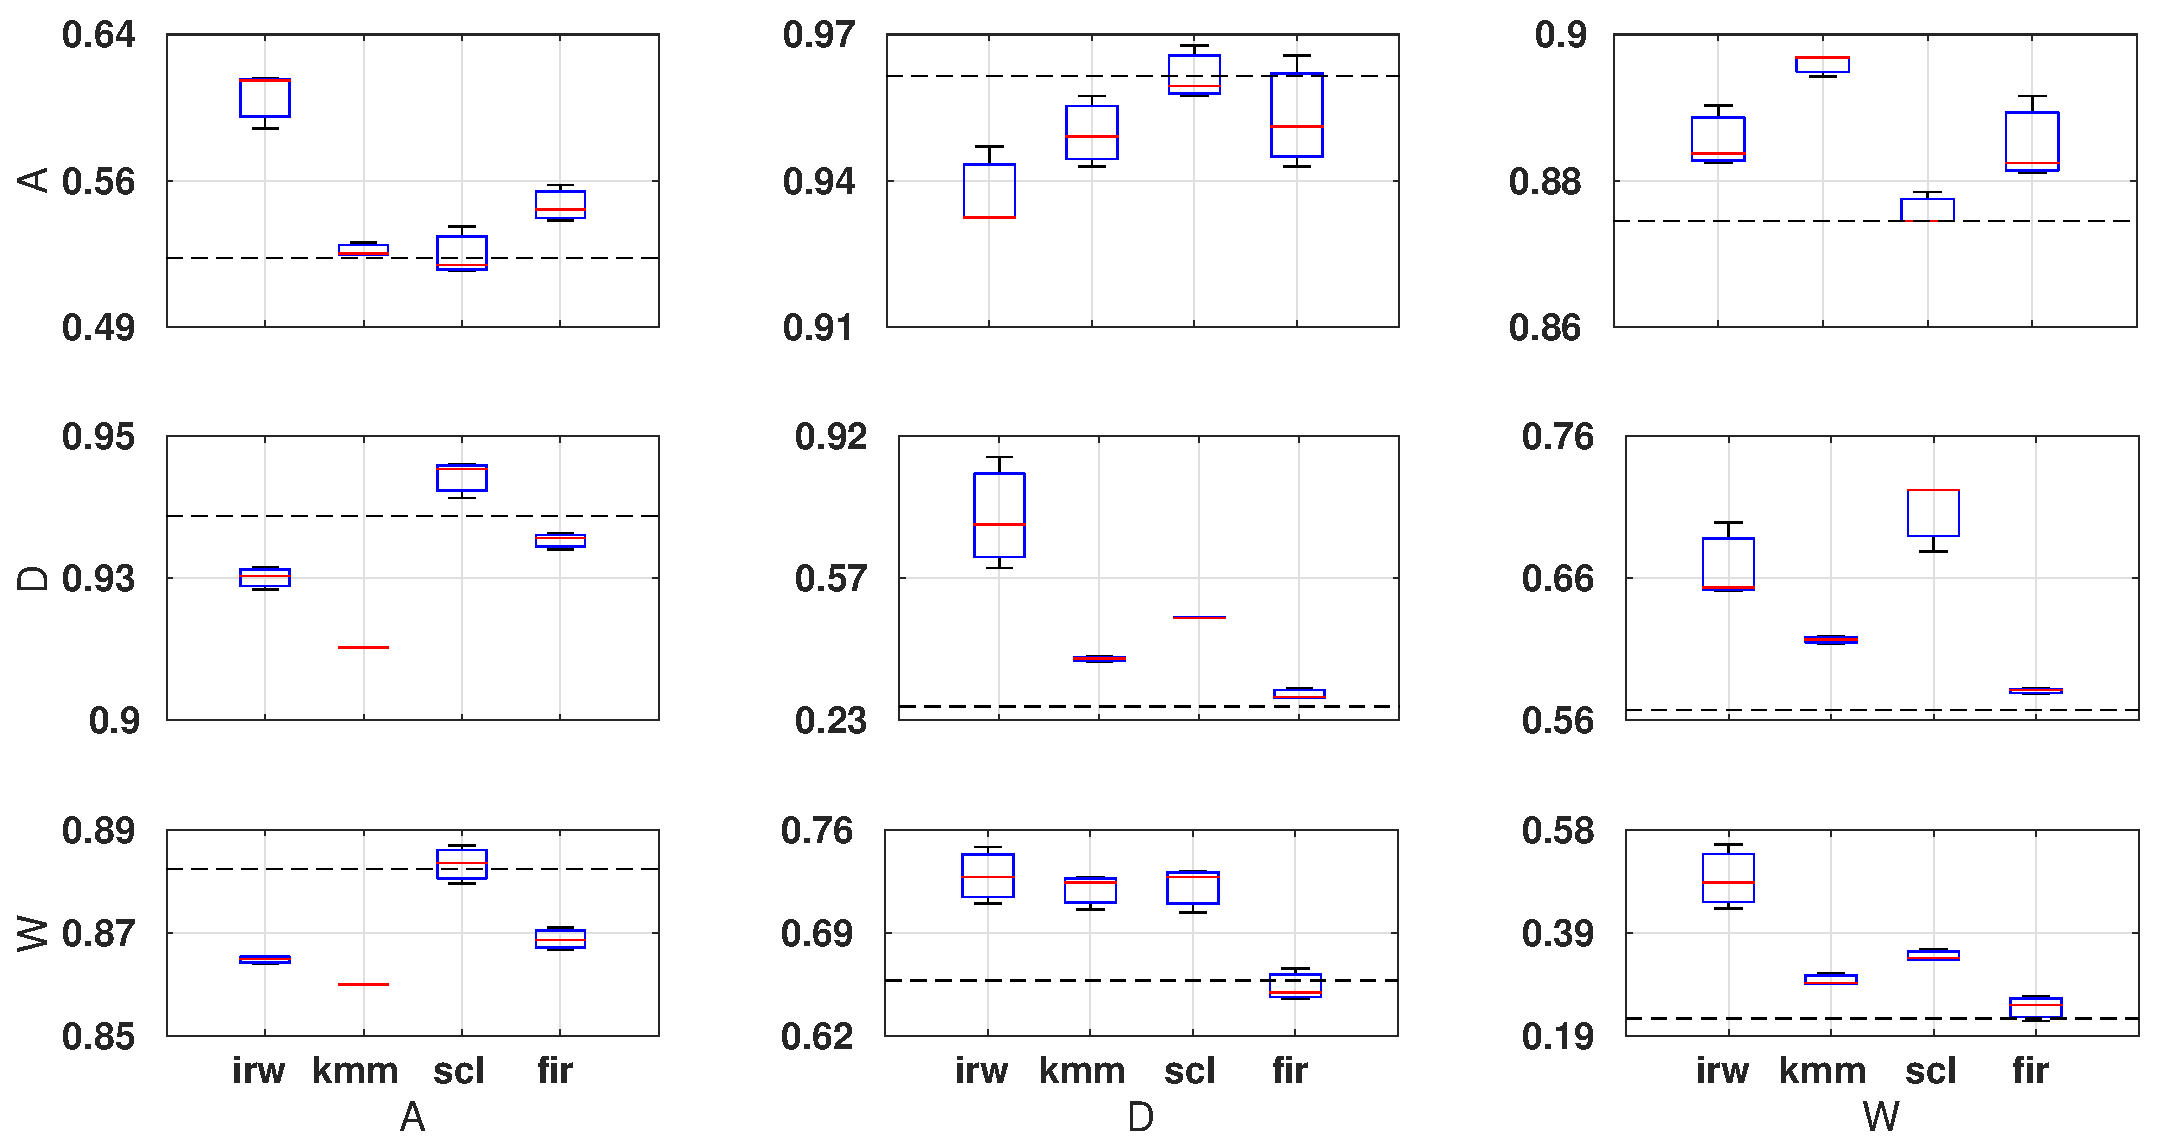
\includegraphics[width=1\textwidth]{images/err_office_box.eps}
	\caption{Box plots of the mean classification error of every repeat of the crossvalidation procedure. The dotted black line is the mean classification error of a naive logistic regressor. Grid shows pairwise combinations of traning on one source domain (rows) and testing on a target domain (columns). A='amazon', D='dslr' and W='webcam'.}
	\label{err_office3}
\end{figure}

Figure \ref{err_office3} once again shows that some pairwise combinations can be successfully adapted to, but for others all classifiers perform nearly at chance level. Kernel mean matching and our fir classifier perform the best for this dataset.

\subsection{Limitations}
Here we look at some limitations of a fir classifier using Bernoulli transfer. Note that these are specific to the transfer distribution.

\subsubsection{Target rate increases}
One thing to consider is to look at when the rate in the target domain is increased. The adapted classifier is not sensitive to this transformation and will predictably revert back to the target classifier. Figure \ref{sens_rateinc} shows that the classifier is behaving as predicted. Methods that rely on learning a domain-invariant representation will not fail in this scenario.

\begin{figure}[ht]
	\centering
	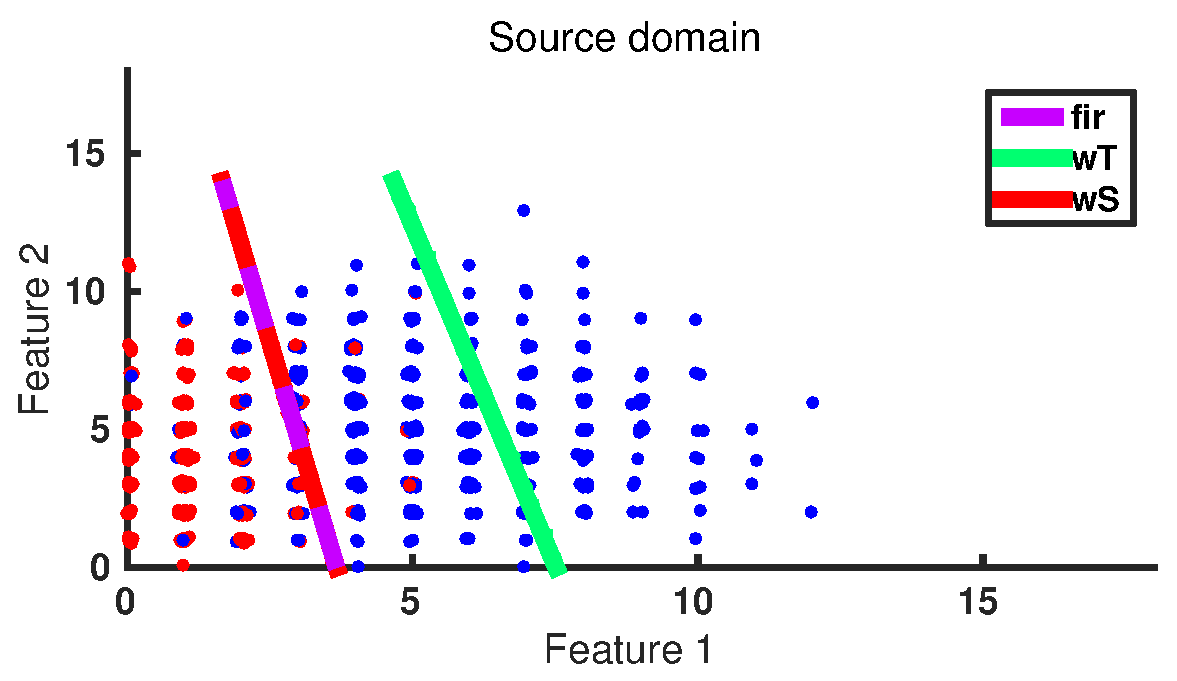
\includegraphics[width=.48\textwidth]{images/da_artexp_rateinc_Poisson_s.eps}
	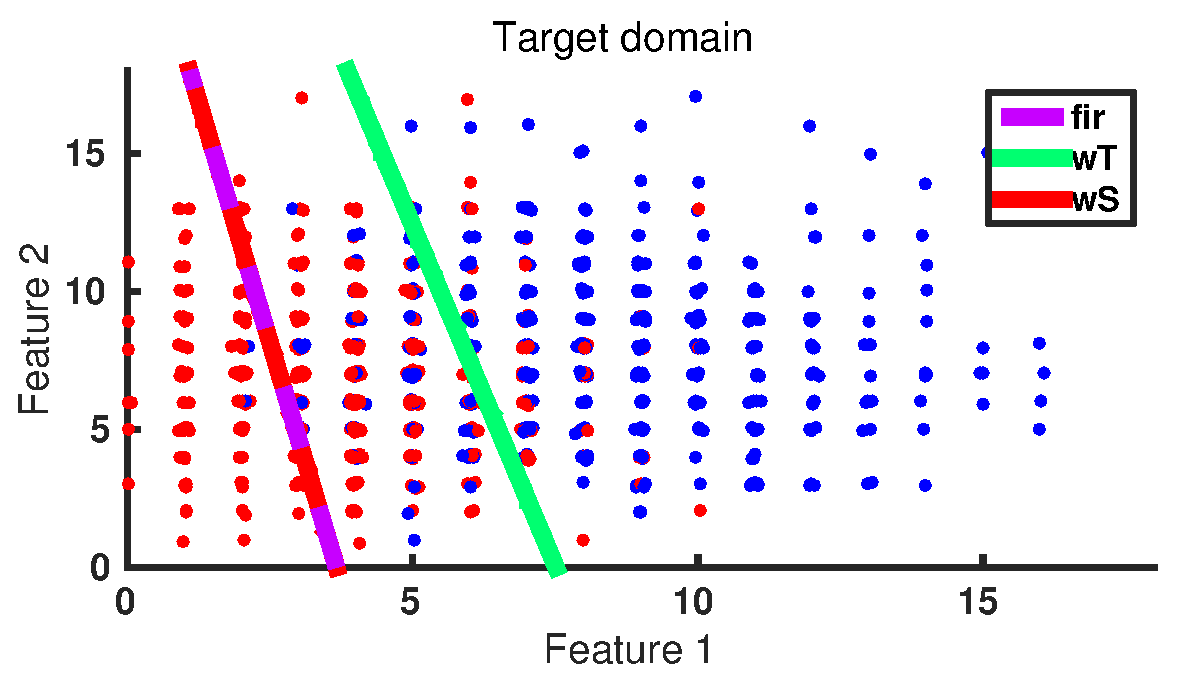
\includegraphics[width=.48\textwidth]{images/da_artexp_rateinc_Poisson_t.eps}
	\caption{Dropout and blankout transfer distributions can not capture increases in the frequency of word use.}
	\label{sens_rateinc}
\end{figure}

\subsubsection{Rate-invariant transformations}
For this experiment, we are interested in how robust the method is to transformations that only minimally affect the frequency of feature use. Figure \ref{sens_model} shows a newly generated target domain with the same rate parameters as the source domain, but with different class distributions. Note that since the estimated transfer parameters are nearly 0, the adapted classifier returns the same solution as the source classifier.

\begin{figure}[ht]
	\centering
	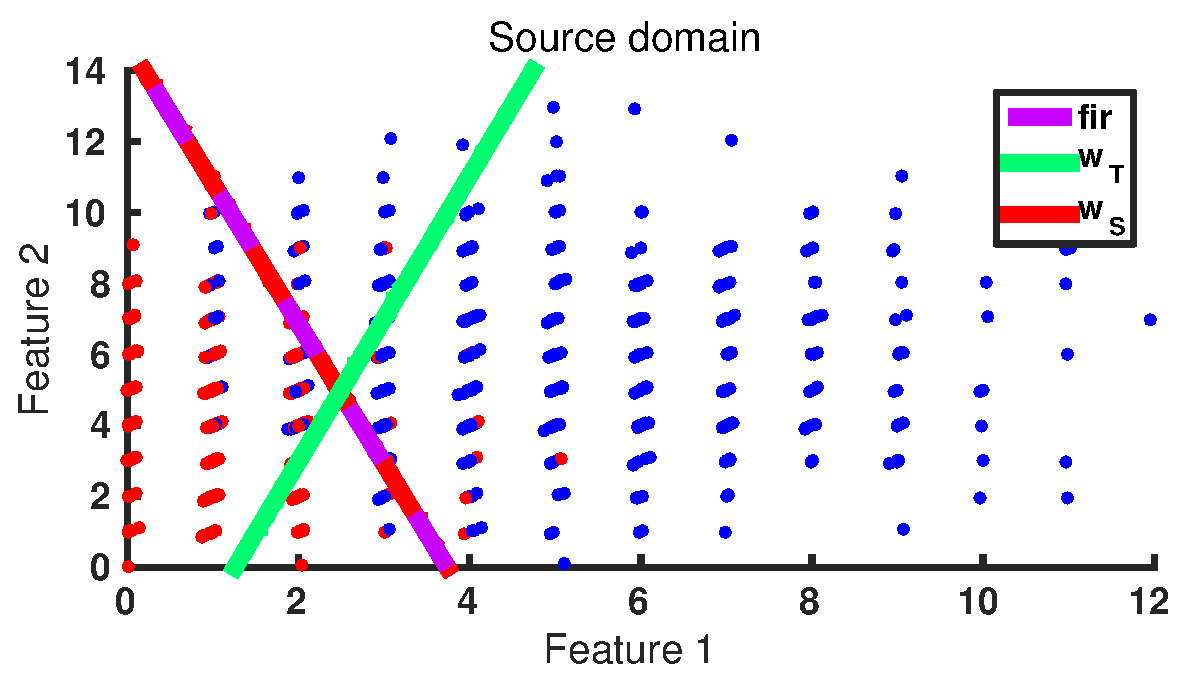
\includegraphics[width=.48\textwidth]{images/da_artexp_sens_model_2.eps}
	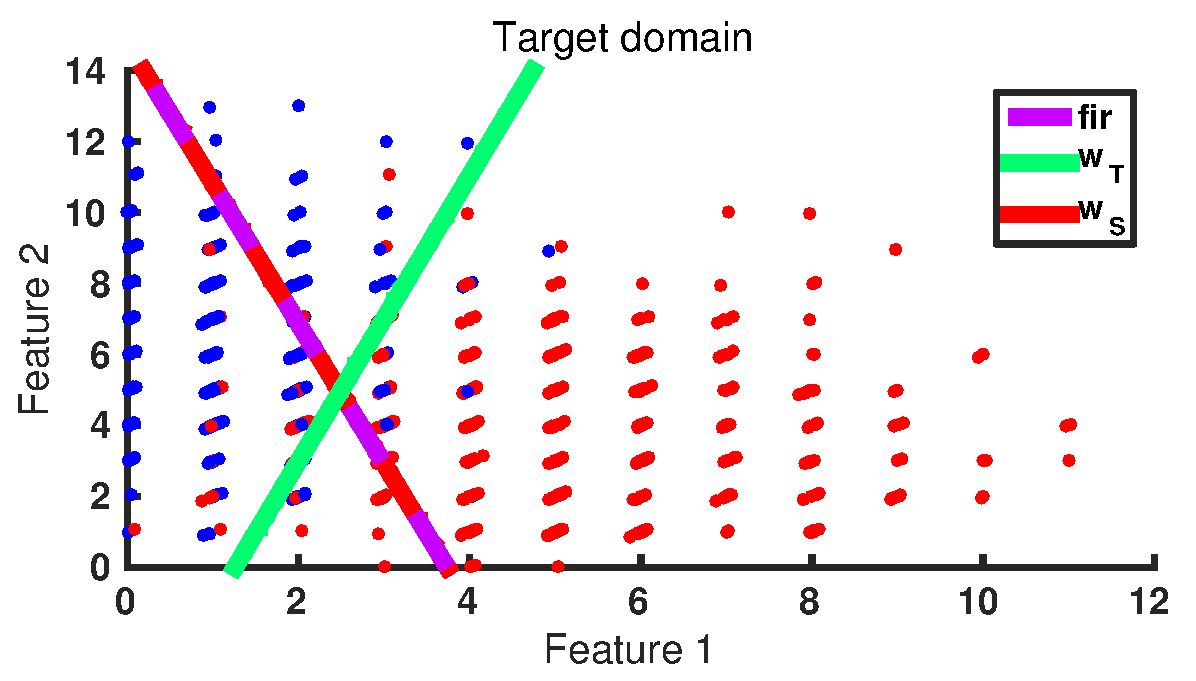
\includegraphics[width=.48\textwidth]{images/da_artexp_sens_model_3.eps}
	\caption{The model is not sensitive to transformations that do not change how much a feature is used.}
	\label{sens_model}
\end{figure}

Note that some of the other models, such as instance reweighting, are also not robust against this type of transformation. Furthermore the more features we capture, the lower the probability of having the same frequency over all features.

\section{Discussion}
For both the quadratic loss and the Taylor approximation of the logistic loss, we can see that the adapted classifer results in the loss on the source samples plus a data-dependent regularization term. It is interesting to consider that regularization is a method of incorporating prior knowledge of the test set in the risk function. If we believe that the solution is not extremely complex for a test set, we employ $\ell_{2}$ regularization, while if we have reason to believe that solution is supposed to be sparse, we can employ $\ell_{!}$ regularization. Since we are looking at very specific test sets here with accompanying data, it makes sense to incorporate our knowledge of the differences in both domains in the regularization term.

Note that for independent domains, the transfer distribution does not exist. Successfully adapting a classifier is arguably not possible for these problems. We do not know in advance if two domains are independent, but one sufficient condition would be if if both domains lived in disjoint subspaces of the feature space. The spam dataset we presented here is an example where it turned out that the two domains, mail and sms, are most likely independent.

Our model is conservative in the sense that if a feature is more present, the corresponding parameter of the transfer distribution is estimated to be $0$ and our classifier reverts to a naive classifier. In the event that a common feature is not discriminative in the source domain but is discriminative in the target domain, we still can not estimate that this feature is necessary. Since we have no knowledge of the target labels, we can not find out whether it will be discriminative then. Note that features that are used extensively but are not discriminative, do not receive a large weight from the classifier any way. Therefore, those do not need to be regularized additionally. 

\section{Conclusion}
In this work we propose an approach to domain adaptation problems that assumes that the posterior over labels transforms along with the data. We propose a transformation based on the relative importance of a feature in the target domain and we show that the resulting classifier can converge to the target classifier. Futhermore, it competes well with some other dominant adaptation strategies.

Future work will focus on an exploration of which transfer distributions are possible, likely and useful. We also aim to extend the current method to continuous data.

% Acknowledgements should go at the end, before appendices and references

\acks{This work was supported by the Netherlands Organization for Scientific Research (NWO; grant 612.001.301).}

%\appendix
%\section*{Appendix A.}


\vskip 0.2in
\bibliography{kouw15a}

\end{document}